\chapter{Evaluation and Analysis}
\label{chapter:evaluation}

In this chapter, we present the results for various models on three datasets---a proprietary dataset provided by a Czech-based company and two open-source datasets (Firefox\footnote{\url{https://www.mozilla.org/firefox/}} and Netbeans\footnote{\url{https://netbeans.org/}}).

We begin the chapter with a process overview where we explain our evaluation flow. In the next section, we provide a description and origin of the used datasets, we also analyze the distribution of our datasets and run two statistical tests to determine how similar the different datasets are.

Our evaluation starts with baseline model which is used to determine whether our models' performance is significantly better than selection of the most frequent developer. Next, we validate the presumption that stop-words removal is advantageous for all our models and in the next section, we finally compare our models. This includes comparison of open source data downloaded from the Internet with the proprietary data provided by a private company. The second to last section contains comparison of the datasets in terms of performance. In our last section, we show how the performance changes for different number of top recommendations.

At the end of the chapter, we continue our work with the window size analysis (and its effect on performance) and we conclude the chapter with the study of topic distribution where we investigate its change over time.

We visualize a lot of the results with plots in this chapter. Because there is a lot of them and we do not want to overwhelm the reader with unnecessary information, we chose to place some of them in appendix~\ref{appendix:extra-plots}. We also decided not to discuss them as the discussion about the plots we placed in this chapter seems sufficient.

The evaluation and analysis is performed in order to find the best possible ML model for practical application of automatic ticket triage. As a part of this theses, we developed a web application that uses our model to predict assignees based on a provided summary and description of a bug report. The link to the repository of the source code can be found in appendix~\ref{appendix:links}.

\section{Process Overview}

Before we dive into the analysis, we provide a flow chart that presents the general process of our analysis and evaluation (Figure~\ref{fig:model.flowchart}). In this section, we discuss the process overview in detail in order to reduce the effort necessary to reproduce this work.

The process begins by retrieving a dataset from a bug tracking system. The next step is to filter unwanted bug reports from the dataset. All tickets that are unassigned, not fixed or not resolved are removed. There are also sometimes bug reports that are assigned to a universal computer-generated user (e.g. \texttt{nobody@mozilla.org}), we remove these reports as well. Bug reports that are resolved by developers that have not fixed sufficient amount of reports in the past (e.g. 30) are also removed. This allows the ML model to be less complicated while sacrificing only a little accuracy.

Another step is to shuffle the bug reports randomly. This is done solely to achieve more accurate performance results with the cross-validation (CV) set, because using newest date for the CV set while training the model on older data is unfair. In practice, only a few new developers are usually used for prediction before they are placed in the training dataset and the model is retrained.

After the steps above, the process continues by splitting the resulting dataset into two sets---a cross-validation set and a training set. The CV set contains 30\% of the bugs while the training set contains the rest (70\%). There are other cross-validation methods (e.g. n-fold cross-validation), we opted for this one because we shuffle the data before we do the split so it is impossible to get biased model.

The second stage is to train a machine learning model. First, however, it is necessary to run the training dataset through a feature extraction step. This step applies techniques that improve the performance of a machine learning model, e.g. stop-words removal, TF--IDF etc. The next step in this stage is to train a machine learning model (e.g. SVM, NB, CART).

The last stage uses the trained machine learning model to generate prediction results that can be used, for example, to compute various performance metrics. The first step is to (again) apply feature extraction techniques on the CV dataset and then use the trained classifier to predict results.

\begin{sidewaysfigure}
    \centering
        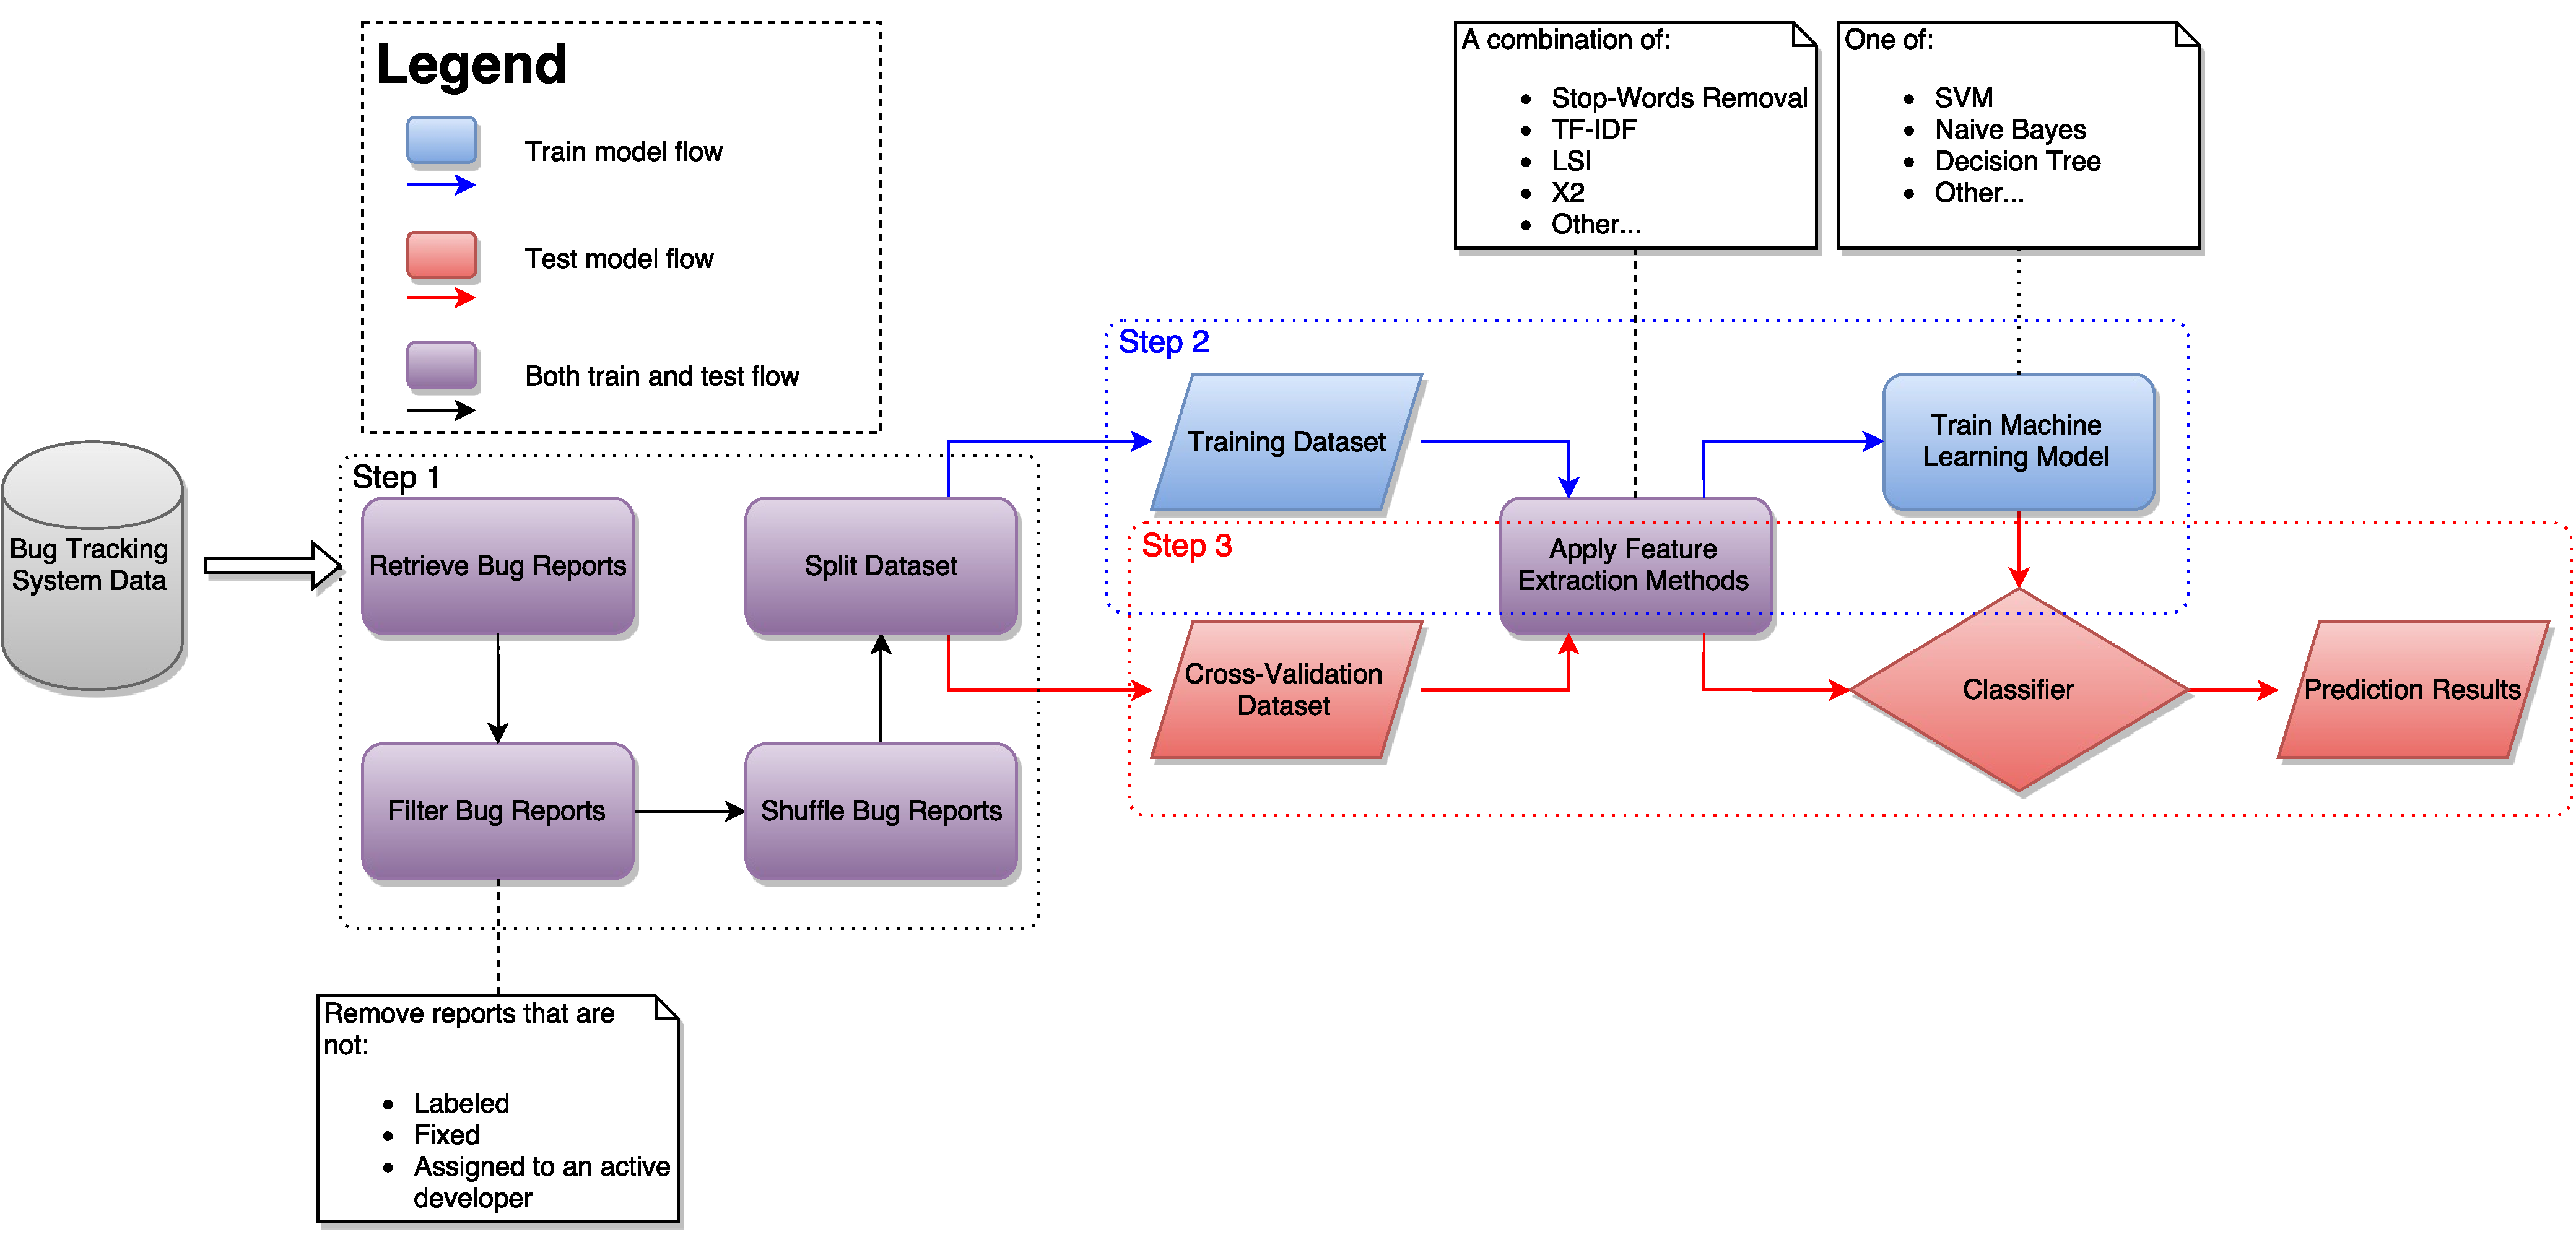
\includegraphics[width=530px, trim=0 5cm 0 0, clip]{./images/flowchart/analysis_flowchart.pdf}
    \caption{Flowchart of the evaluation and analysis process.}
    \label{fig:model.flowchart}
\end{sidewaysfigure}
\clearpage

\section{Datasets}
\label{section:datasets}

To evaluate the performance of a model, we need a set of bug tracking data. One dataset was provided by a private company, but as we eventually want to compare our results with related work, we selected two other open-source projects that are frequently used for training and testing of ML models in related work---Netbeans and Firefox.

In this section, we provide description of these three datasets. We also do a basic analysis of the datasets which will allow us to establish some basic answers to GQM questions \hyperlink{question:4}{4} and \hyperlink{question:5}{5}.

\subsection{Firefox Data}

This dataset is downloaded from Mozilla repository\footnote{\url{https://bugzilla.mozilla.org}} from project Firefox. We downloaded all bugs that are in status \texttt{RESOLVED} with resolution \texttt{FIXED} and were created in year 2010 or later. We also removed bugs with field \texttt{assigned\_to} set to \texttt{nobody@mozilla.org} as those tickets were not assigned to an actual developer.

\begin{figure}[htbp]
    \centering
        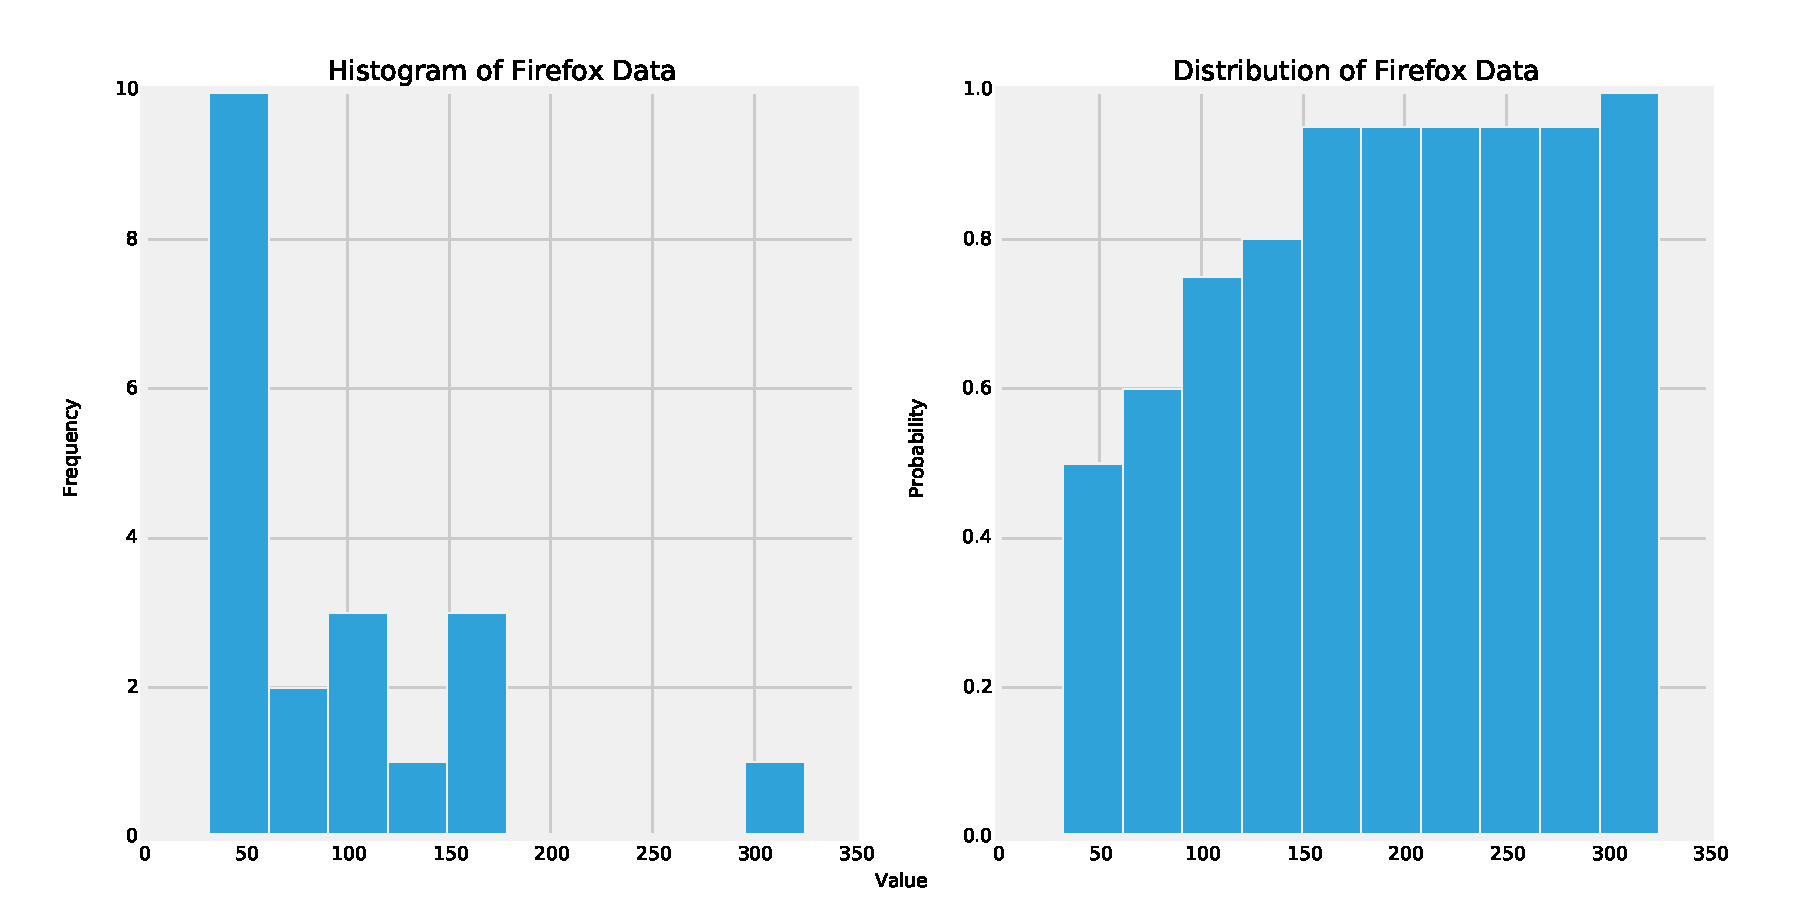
\includegraphics[width=\textwidth]{./images/distribution/firefox.pdf}
    \caption{Histogram and distribution of the Firefox data.}
    \label{fig:datasets.firefox.dist}
\end{figure}

In total, we were able to retrieve $9,141$ bugs. To get a better comparison with the other datasets, we only use $3,000$ datasets for training and cross-validation that were created between 2010-01-01 and 2012-07-10. This dataset contains $343$ labels (developers). Finally, we remove developers who did not fix at least $30$ bugs, yielding $1,810$ bugs with $20$ developers. The histogram with frequencies of the developers and cumulative distribution is on figure~\ref{fig:datasets.firefox.dist}.

\subsection{Netbeans Data}

Netbeans data were downloaded from Netbeans bug repository\footnote{\url{https://netbeans.org/bugzilla/}}. We considered latest $3,000$ bugs that are in status \texttt{RESOLVED} with resolution \texttt{FIXED}. We removed bugs with assignee \texttt{kenai\_tester\_git} (as those were created automatically) resulting in $2,924$ bug reports. These bugs were created between 2014-06-14 and 2015-06-14 and they contain $92$ developers. After removing developers who did not fix at least 30 bugs, the dataset contains $2,528$ reports with $30$ developers. Figure~\ref{fig:datasets.netbeans.dist} is a histogram and distribution of this datasets.

\begin{figure}[htbp]
    \centering
        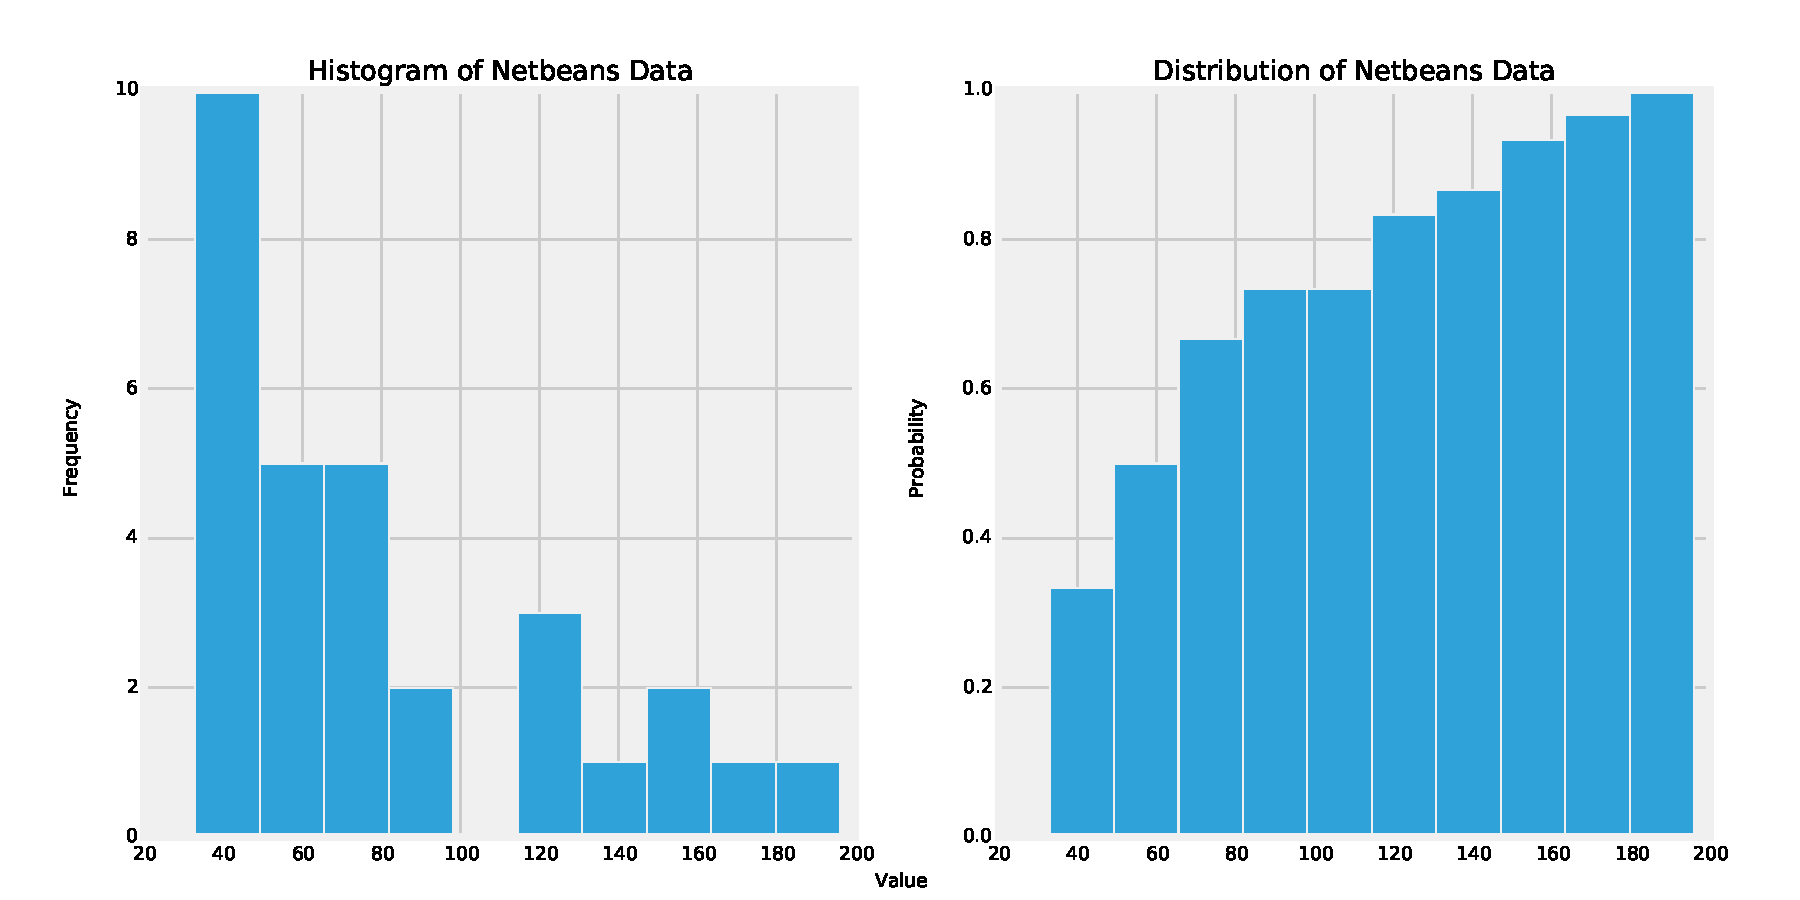
\includegraphics[width=\textwidth]{./images/distribution/netbeans.pdf}
    \caption{Histogram and distribution of the Netbeans data.}
    \label{fig:datasets.netbeans.dist}
\end{figure}

\subsection{Proprietary Data}

The Proprietary dataset was provided by a company that wants to remain anonymous. The provided dataset contains $2,926$ bug reports created between 2012-11-23 and 2015-10-16. Only bug reports that were resolved with assigned developer were considered. There are $110$ developers in this dataset. Only $2,424$ bugs assigned to $35$ developers were retained after removal of developers with less than $30$ fixed bugs. The histogram and probability distribution is pictured on figure~\ref{fig:datasets.proprietary.dist}.

\begin{figure}[htbp]
    \centering
        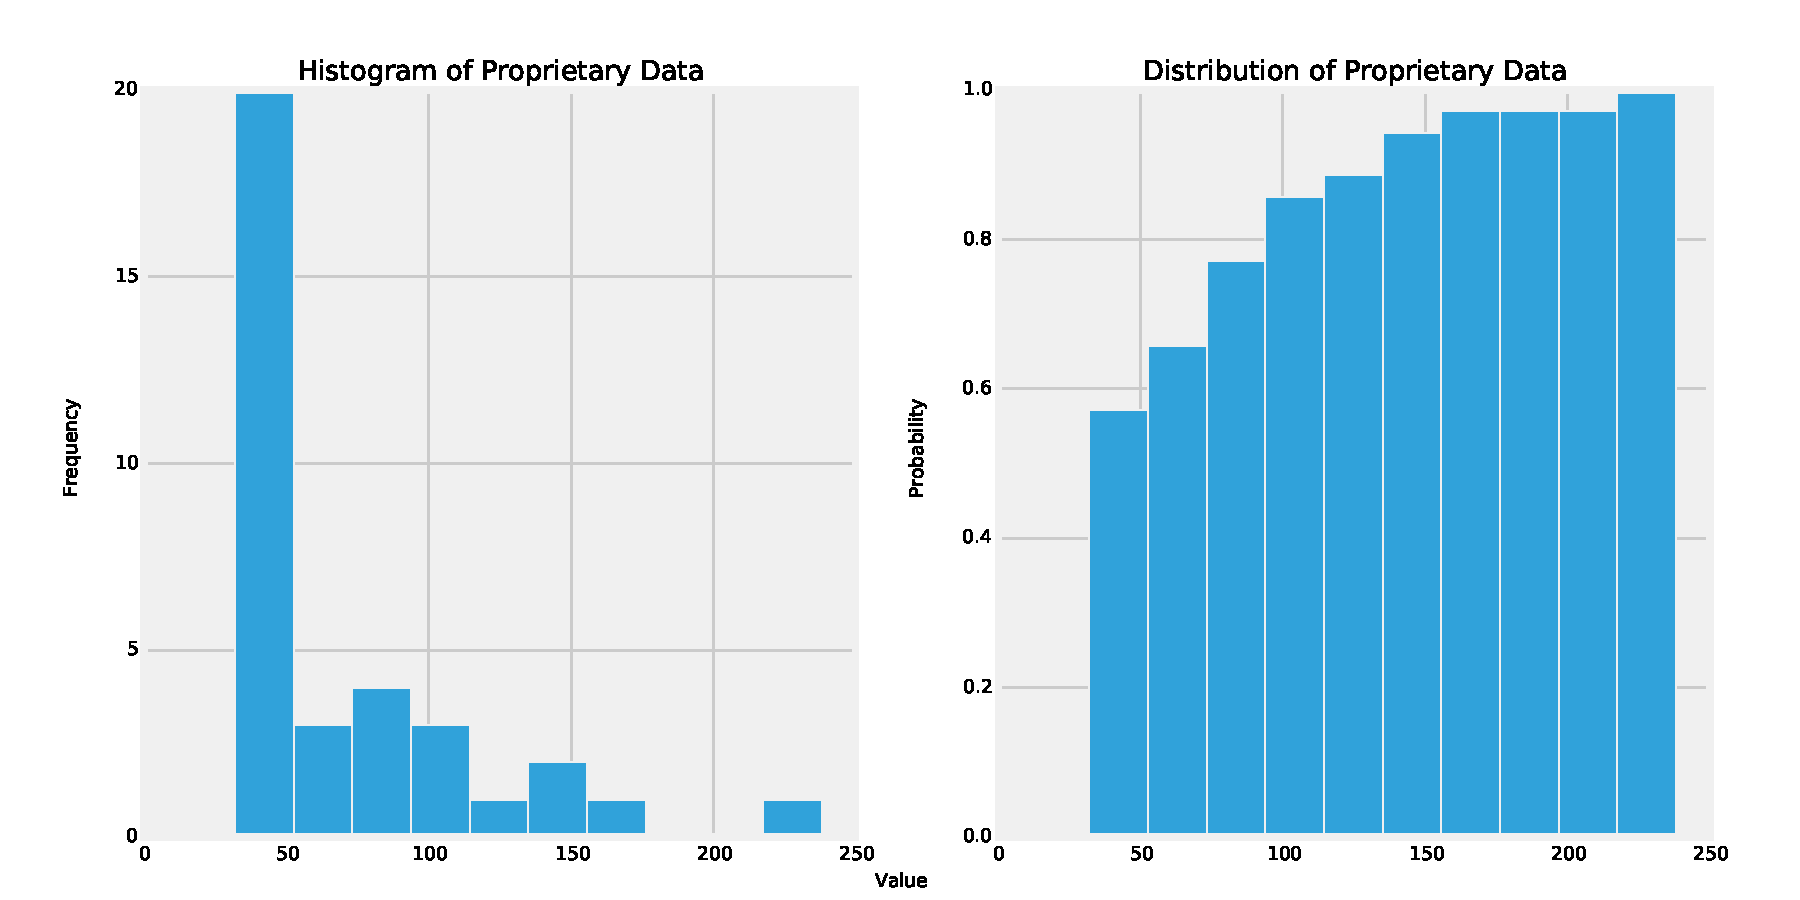
\includegraphics[width=\textwidth]{./images/distribution/proprietary.pdf}
    \caption{Histogram and distribution of the Proprietary data.}
    \label{fig:datasets.proprietary.dist}
\end{figure}

\subsection{Chi-Square Test}

In this section, we test the null hypothesis that two samples are from the same distribution, which will allow us to determine how similar the used datasets are. For this, we use the two-sided alternative of two-sample Chi-Square test. We split the samples from each datasets into five bins and compute the \textit{p-value} for three pairs of samples.

The Chi-Square test with Netbeans and Firefox samples yields p-value of $0.4283$, as p-value~$> 0.05$ we fail to reject the null hypothesis that the two samples are from the same distribution with 5\% level of significance.

The test with Firefox and Proprietary samples returns p-value equal to $0.8648$ so we again fail to reject the null hypothesis. The last test with samples from Proprietary and Netbeans data results in p-value of $0.6182$, which again means the null hypothesis cannot be rejected (with 5\% significance).

\subsection{T-Test}

In the previous section, we tested the hypothesis that the datasets used in this thesis are from the same distribution. We failed to reject the hypothesis with all samples, in this section, we test the null hypothesis that the samples have the same population mean---allowing us to futher learn how statistically similar the datasets are. For that, we have to test the hypothesis that the variances of the samples are the same.

We use the two-sided alternative of the standard independent two-sample t-test to test the null hypothesis that the samples have the same population mean, and the two-sided alternative of the Levene test to test whether the samples have equal population variance. If we reject the null hypothesis of the Levene test, we use the two-sided alternative of the Welch's t-test instead of the standard variant.

First, we test the samples from Firefox and Proprietary datasets. The Levene test yields p-value equal to $0.2730$, as p-value~$> 0.05$, we fail to reject the null hypothesis with 5\% significance level. To test the population mean of the two samples, we therefore have to use the standard independent t-test. The standard independent t-test results in p-value of $0.1954$, which means we fail to reject the null hypothesis of equal population mean of the two samples with 5\% significance.

Second, we test the samples from Firefox and Netbeans repositories. As the Levene test returns p-value equal to $0.4397 > 0.05$, we fail to reject the null hypothesis of equal population variances (5\% significance). The p-value of the standard independent t-test on these two samples is equal to $0.5924$, which means we fail to reject the null hypothesis of equal population means with 5\% significance.

Last samples we test are from Netbeans and Proprietary datasets. The p-value of the Levene test for these two samples is $0.6007$ thus we fail to reject the null hypothesis of equal variances. The p-value of the standard independent t-test is equal to $0.3061$, which again means we have to reject the null hypothesis that the two samples have the same population mean (5\% significance).

\subsection{Conclusion}

Our basic analysis of the datasets allows us to partially answer two questions established in chapter~\ref{chapter:methodology}. The similarity in the distributions and means of the datasets suggests that our models will work on all datasets regardless of parameter values (\hyperlink{question:4}{Q4}). The results of our chi-square test and t-test imply there is little difference between proprietary and open-source data, partially answering~\hyperlink{question:5}{Q5}. Our confidence in these answers will be further refined when we evaluate our models and datasets.

\section{Baseline}
\label{section:baseline}

In this section, we establish a baseline for our models (addressing~\hyperlink{question:1}{Q1}). Our baseline is very simple, the number of bug report that is assigned to each developer is counted and the developer with the highest number of assigned bugs is selected as a prediction for each subsequent call of the \texttt{predict} function.

Figure~\ref{fig:models.firefox.stopwords} shows the performance of the baseline model on Firefox data. While the accuracy of this model is relatively high (18\%), the precision and recall values are much lower (1\% and 5\%), which can be explained by the way macro-averaged metrics work, see metrics in chapter~\ref{chapter:methodology}. The results for the other two datasets are available in appendix~\ref{appendix:extra-plots}.

\begin{figure}[htbp]
    \centering
        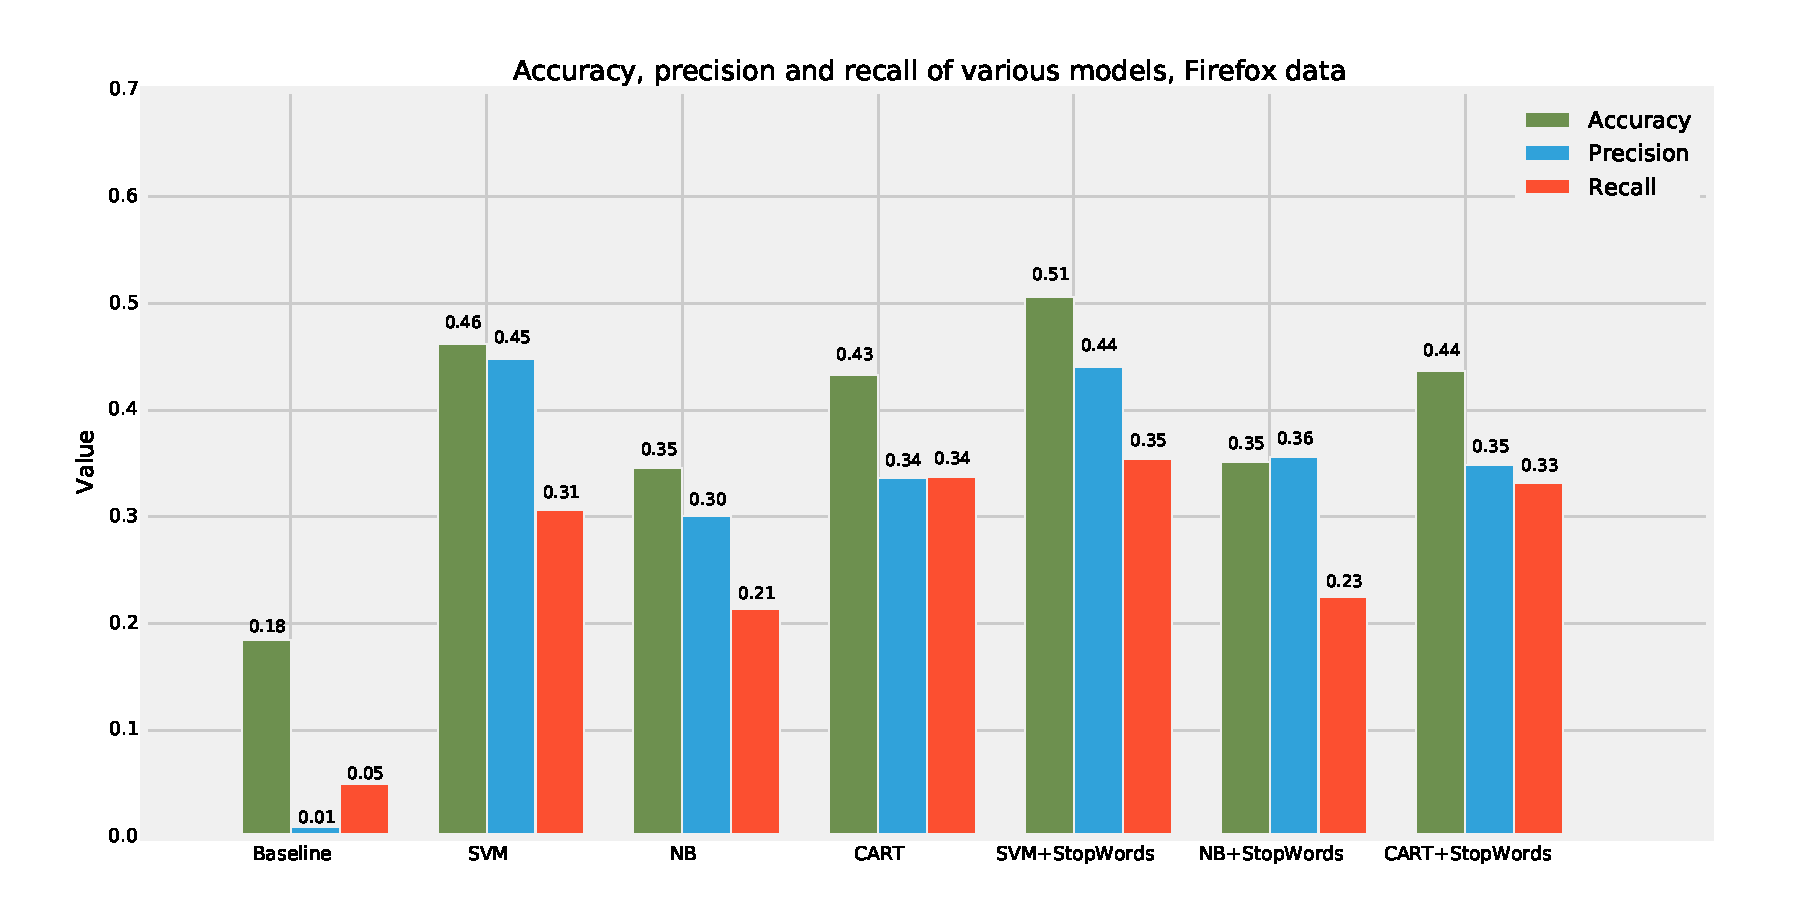
\includegraphics[width=\textwidth]{./images/comparison_of_models/firefox_0.pdf}
    \caption{Baseline and stop-words removal results comparision on Firefox data.}
    \label{fig:models.firefox.stopwords}
\end{figure}

\section{Stop-Words Removal}

Stop-words removal is a technique that can increase performance of a ML model. In this section, we determine whether the increase is significant enough to warrant its usage for subsequent comparisons of models.

Figure~\ref{fig:models.firefox.stopwords} shows the increase in performance after all stop-words were removed from the feature vector of the Firefox data. You can see that the performance of the classifier slightly increased on all models. Accuracy increased by 3\%, 0\% and 1\% on SVM, Naive Bayes and CART model respectively. Precision value of the SVM model decreased by 1\% but increased by 6\% with Naive Bayes model and by 1\% with CART. Finally, Recall values of SVM and Naive Bayes increased by 4\% and 2\% respectively while it slightly decreased with the CART model by about 1\%.

The results of the other datasets were similar in nature (See appendix~\ref{appendix:extra-plots}). We therefore conclude that the performance boost of stop-words removal is significant enough to warrant better results, which matches the conclusion of Čubranić and Murphy~\cite{Murphy} (see chapter~\ref{chapter:related-work}). Thus, in our evaluation, we always use stop-words removal in combination with other feature extraction methods.

\section{Comparison of Models}

In the following text, comparison of the ML models is presented. We show the \hyperlink{metric:a}{accuracy}, \hyperlink{metric:p}{precision} and \hyperlink{metric:r}{recall} of these models on the three datasets. Based on related work (chapter~\ref{chapter:related-work}), we decided to compare three models---Naive Bayes, CART and Support Vector Machine. The theoretical background of these models is covered in chapter~\ref{chapter:background}. The metrics we use are explained in chapter~\ref{chapter:methodology}. The parameters of all models were optimized using grid search\footnote{\url{http://scikit-learn.org/stable/modules/grid\_search.html}}.

In terms of GQM, this section attempts to answer question~\hyperlink{question:2}{2} (how many times the model predicts the correct assignee), question~\hyperlink{question:3}{3} (how often the model predicts the correct assignee if the distribution of bug reports is unbalanced) and question~\hyperlink{question:4}{4} (if the model with the same parameters works with all projects). The answers are addressed in the conclusion of this section.

\subsection{Firefox Data}

On Figure~\ref{fig:results.models.firefox}, you can see the performance of the chosen models on Firefox data. The SVM model with TF--IDF weighing achieves the best performance with accuracy of 57\%. Its precision and recall also outperforms all the other approaches with values of 51\% and 45\%. The same model with LSI takes second place. The only model other than SVM that approaches SVM with it's performance is CART, especially with TF--IDF weighing.

\begin{figure}[htbp]
    \centering
        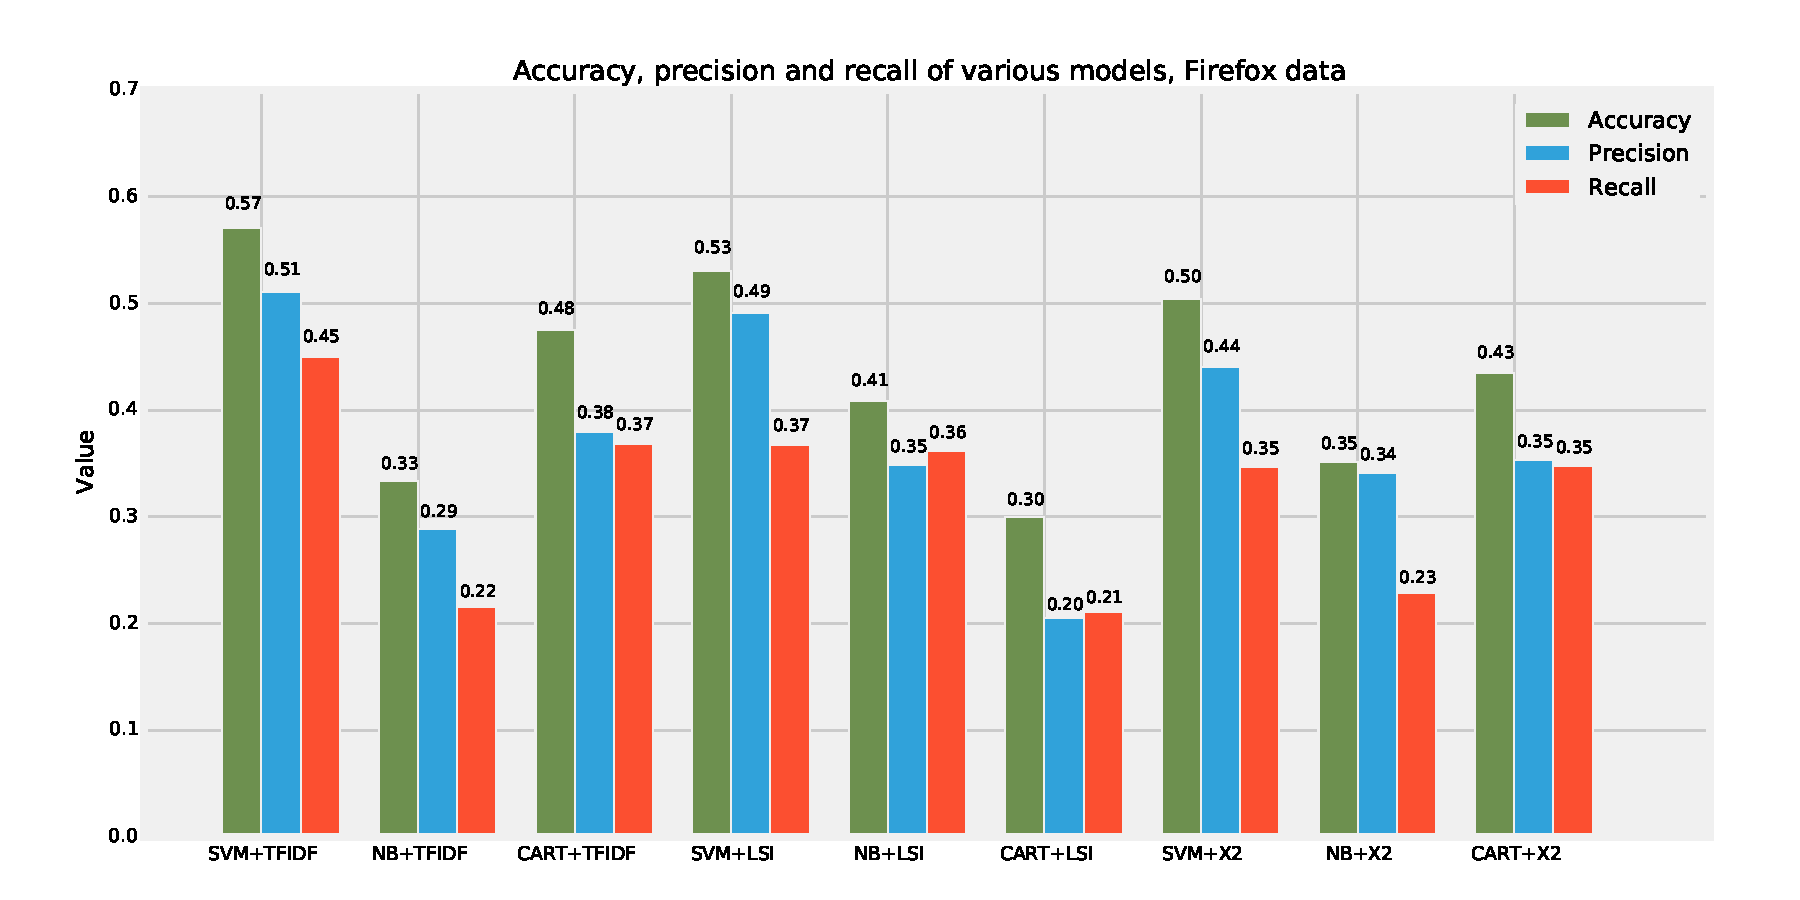
\includegraphics[width=\textwidth]{./images/comparison_of_models/firefox.pdf}
    \caption{Comparison of models on Firefox data.}
    \label{fig:results.models.firefox}
\end{figure}

\subsection{Netbeans Data}

The performance of the models on Netbeans data is shown on Figure~\ref{fig:results.models.netbeans}. It is clear that the SVM model with TF--IDF weighing performs best even on the Netbeans data, although in this case the LSI feature extraction technique does not seem to perform as well as in the previous case. The accuracy, precision and recall of the approach are 53\%, 53\% and 49\% respectively. Sole SVM model and SVM+$\chi^2$ model perform similarly as far as precision is concerned, while the accuracy and recall values are lagging behind by a considerable margin. None of the other models offer better performance than even sole SVM model on this data, which suggests that SVM is a very good choice for automatic bug assignment.

\begin{figure}[htbp]
    \centering
        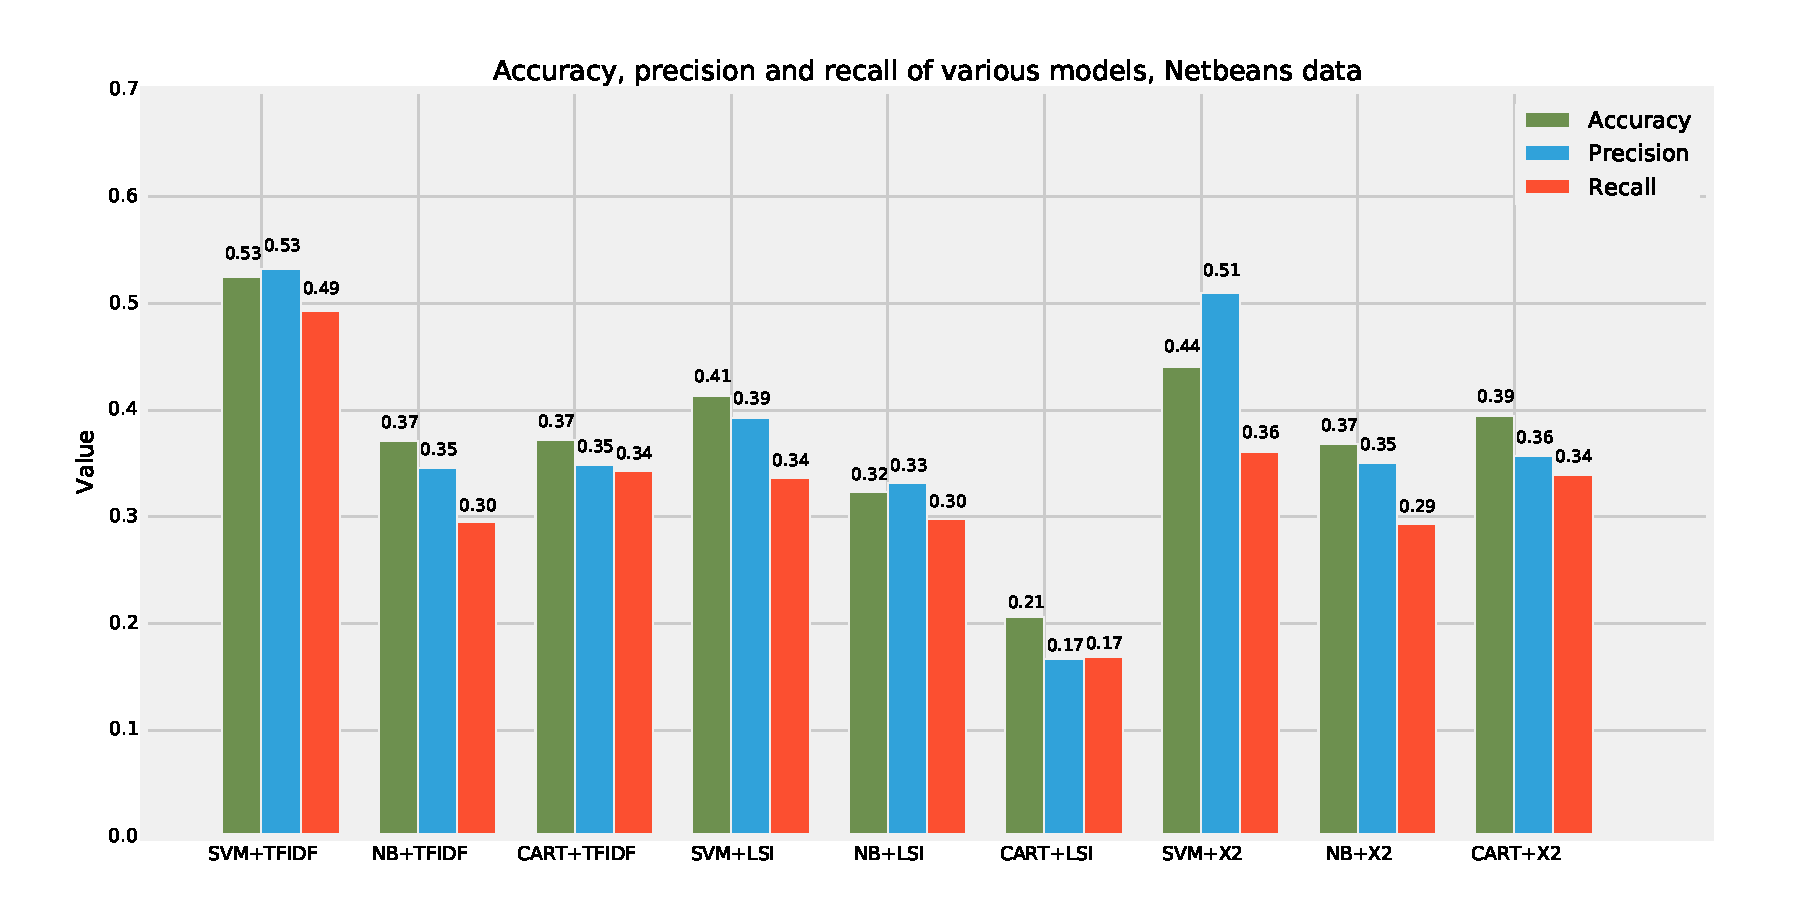
\includegraphics[width=\textwidth]{./images/comparison_of_models/netbeans.pdf}
    \caption{Comparison of models on Netbeans data.}
    \label{fig:results.models.netbeans}
\end{figure}

\subsection{Proprietary Data}

The proprietary data results are similar to the open-source datasets. Even in this case, the SVM model with TF--IDF offers the best performance of 53\% accuracy, 59\% precision and 47\% recall. The same model with LSI also shows quite good performance and rather surprisingly, the Naive Bayes model with $\chi^2$ and TF--IDF performs quite well as far as precision is concerned. Both SVM and Naive Bayes models exhibit rather wide spreads between precision and recall values, which could be an indication of higher variance of the proprietary data (the distribution chart in section~\ref{section:datasets} seems to support this statement). Figure~\ref{fig:results.models.proprietary} presents the results in a graphical manner.

\begin{figure}[htbp]
    \centering
        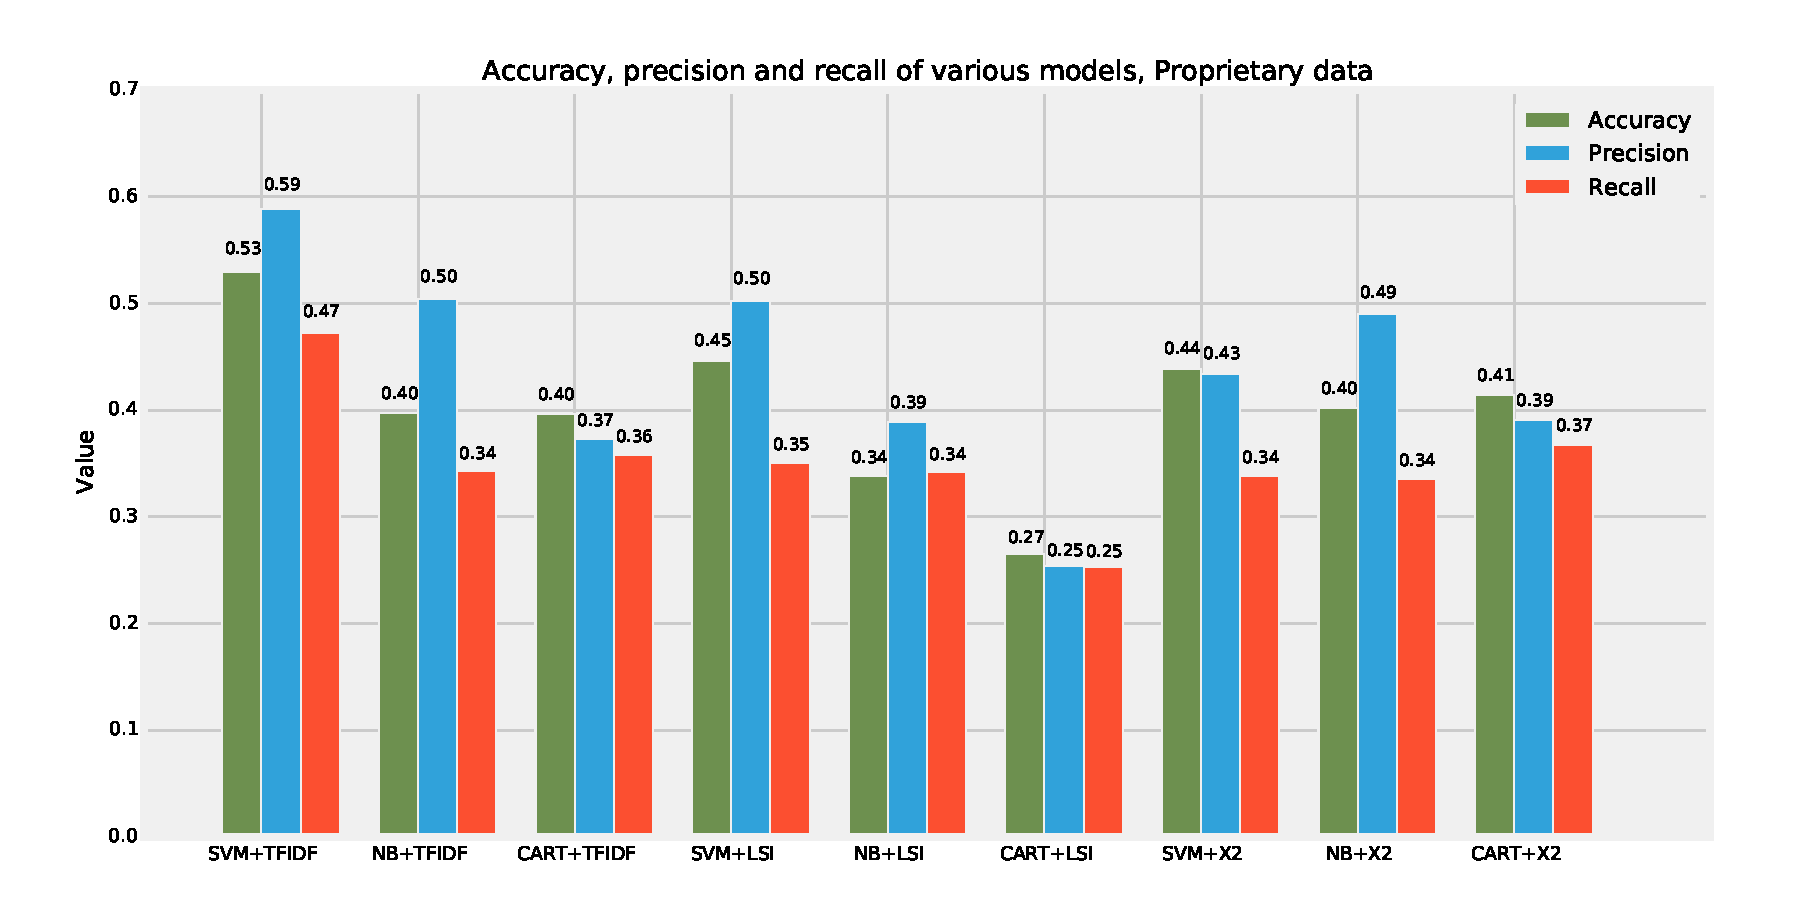
\includegraphics[width=\textwidth]{./images/comparison_of_models/proprietary.pdf}
    \caption{Comparison of models on the Proprietary data.}
    \label{fig:results.models.proprietary}
\end{figure}

\subsection{Conclusion}

The comparison shows that SVM with TF--IDF weighing performs best on all datasets. Not only that, it also generalizes very well, because there was no need to readjust the parameters of the model to get the best or nearly the best performance for all datasets. The disadvantage of the model is that it is the most computationally complex one, because SVM is the slowest of the three models as there are a lot of classes and features. This can be at least partially dealt with by using $\chi^2$ feature extraction in conjunction with TF-IDF while sacrificing some of the performance.

The accuracy of all our models shows us how many times they are able to predict the correct assignee (\hyperlink{question:2}{Q2}). The precision and recall values of these models indicate that the models perform well even for unbalanced data (\hyperlink{question:3}{Q3}), there is, however, slight bias towards higher precision than recall. While the SVM model does not need different settings for different datasets and the NB and CART models do not have any, both LSI and $\chi^2$ feature extraction methods need to be tuned for each dataset to achieve the best performance (\hyperlink{question:4}{Q4}). It is therefore apparent that the SVM model with TF--IDF has a huge advantage over all the other models we tested.

\section{Comparison of Datasets}
\label{section:comparison-of-datasets}

The main purpose of this section is to compare the proprietary dataset with the open-source datasets, providing an answer to question~\hyperlink{question:5}{5} of our application of GQM described in chapter~\ref{chapter:methodology}. In this section, we compare the proprietary dataset with only the Firefox dataset and we only use the Naive Bayes with no feature extraction method other than stop-words removal, and SVM model with TF--IDF weighing.

We compare these two datasets by computing their performance (accuracy, precision and recall) for six different settings of the minimum \textit{issues per developers} requirement. These settings are: 1, 3, 5, 10, 20, 30. This allows us to see how the performance of the datasets changes when different number of developers (and bugs assigned to them) are removed. The narrower is the difference of the performance between the datasets for all the setting values, the higher is our confidence there is not much difference between open-source and proprietary data.

\subsection{Naive Bayes Model}

The first model for comparison is Naive Bayes. The only used feature extraction method for this model is stop-words removal, as we mentioned above.

\begin{figure}[htbp]
    \centering
        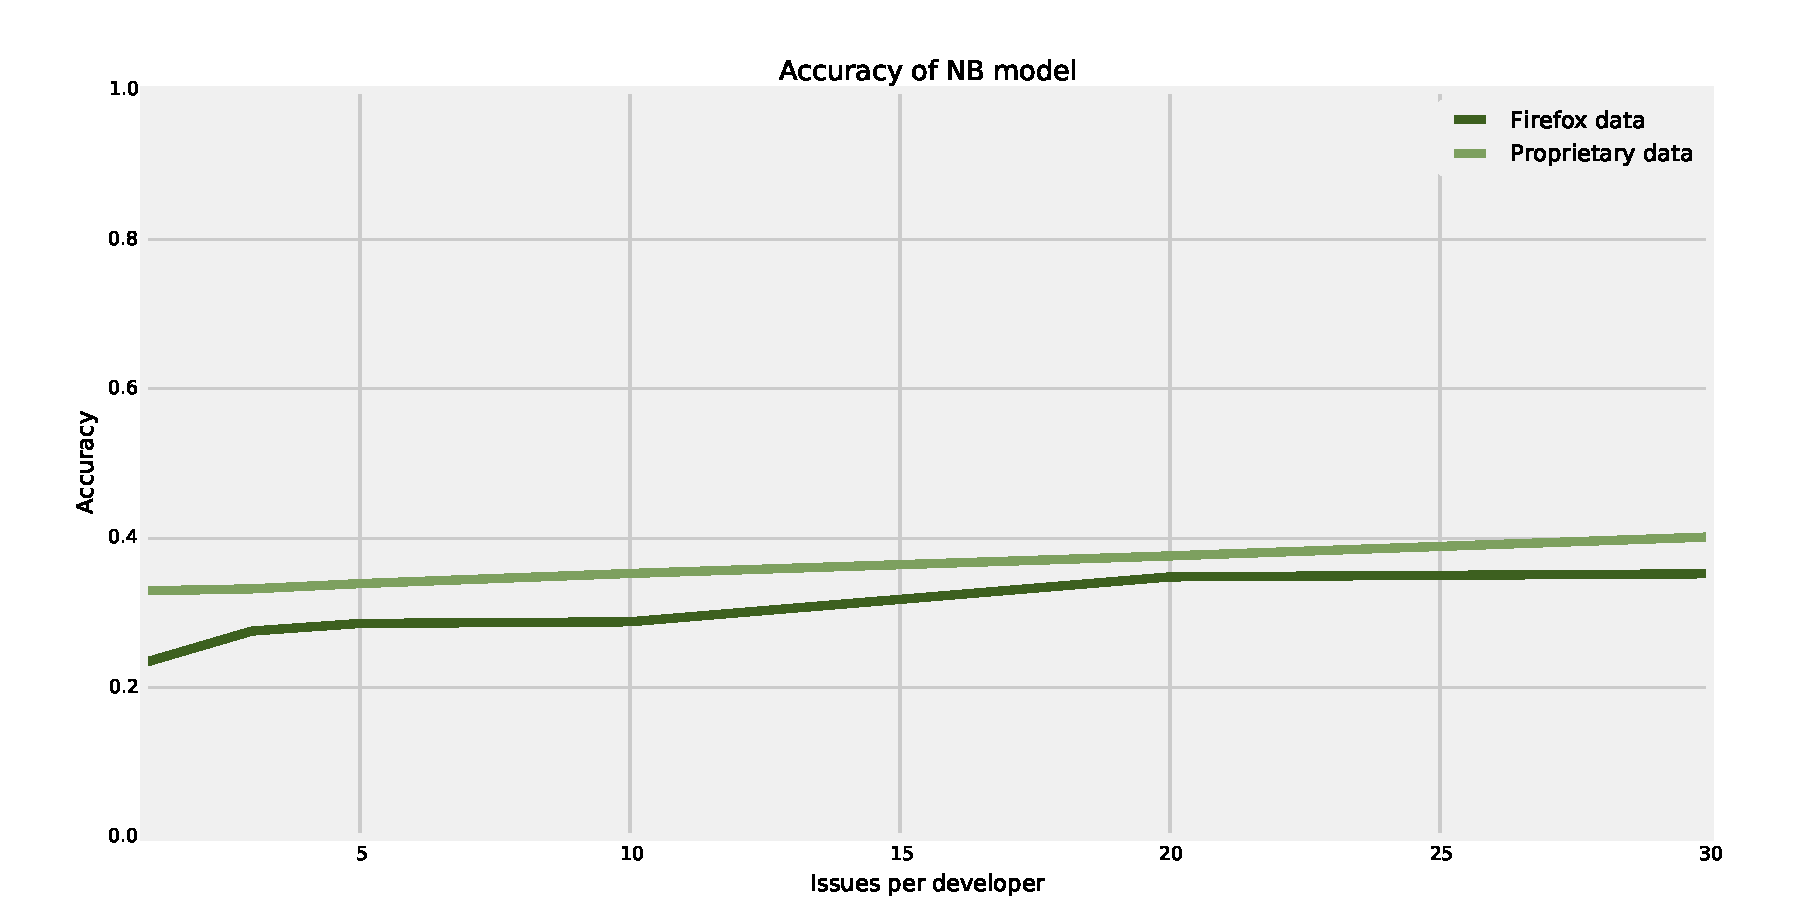
\includegraphics[width=\textwidth]{./images/prop_vs_os/nb_accuracy.pdf}
    \caption{Comparison of accuracy of Naive Bayes model.}
    \label{fig:results.datasets.nb_accuracy}
\end{figure}

First plot (Figure \ref{fig:results.datasets.nb_accuracy}) represents accuracy of the Naive Bayes model. You can see there are some interesting differences between the performances of the proprietary and open-source datasets. When the minimum requirement for issues per developer is 1, the accuracy of the proprietary dataset (33\%) is significantly higher than the accuracy of the open-source dataset (23\%). On the other hand, the accuracy of the proprietary dataset is higher for all settings of minimum issues per developer. When the requirement of issues per developers increases to 30, there is only 5\% difference between the accuracy of the proprietary dataset (40\%) and the open-source dataset (35\%).

\begin{figure}[htbp]
    \centering
        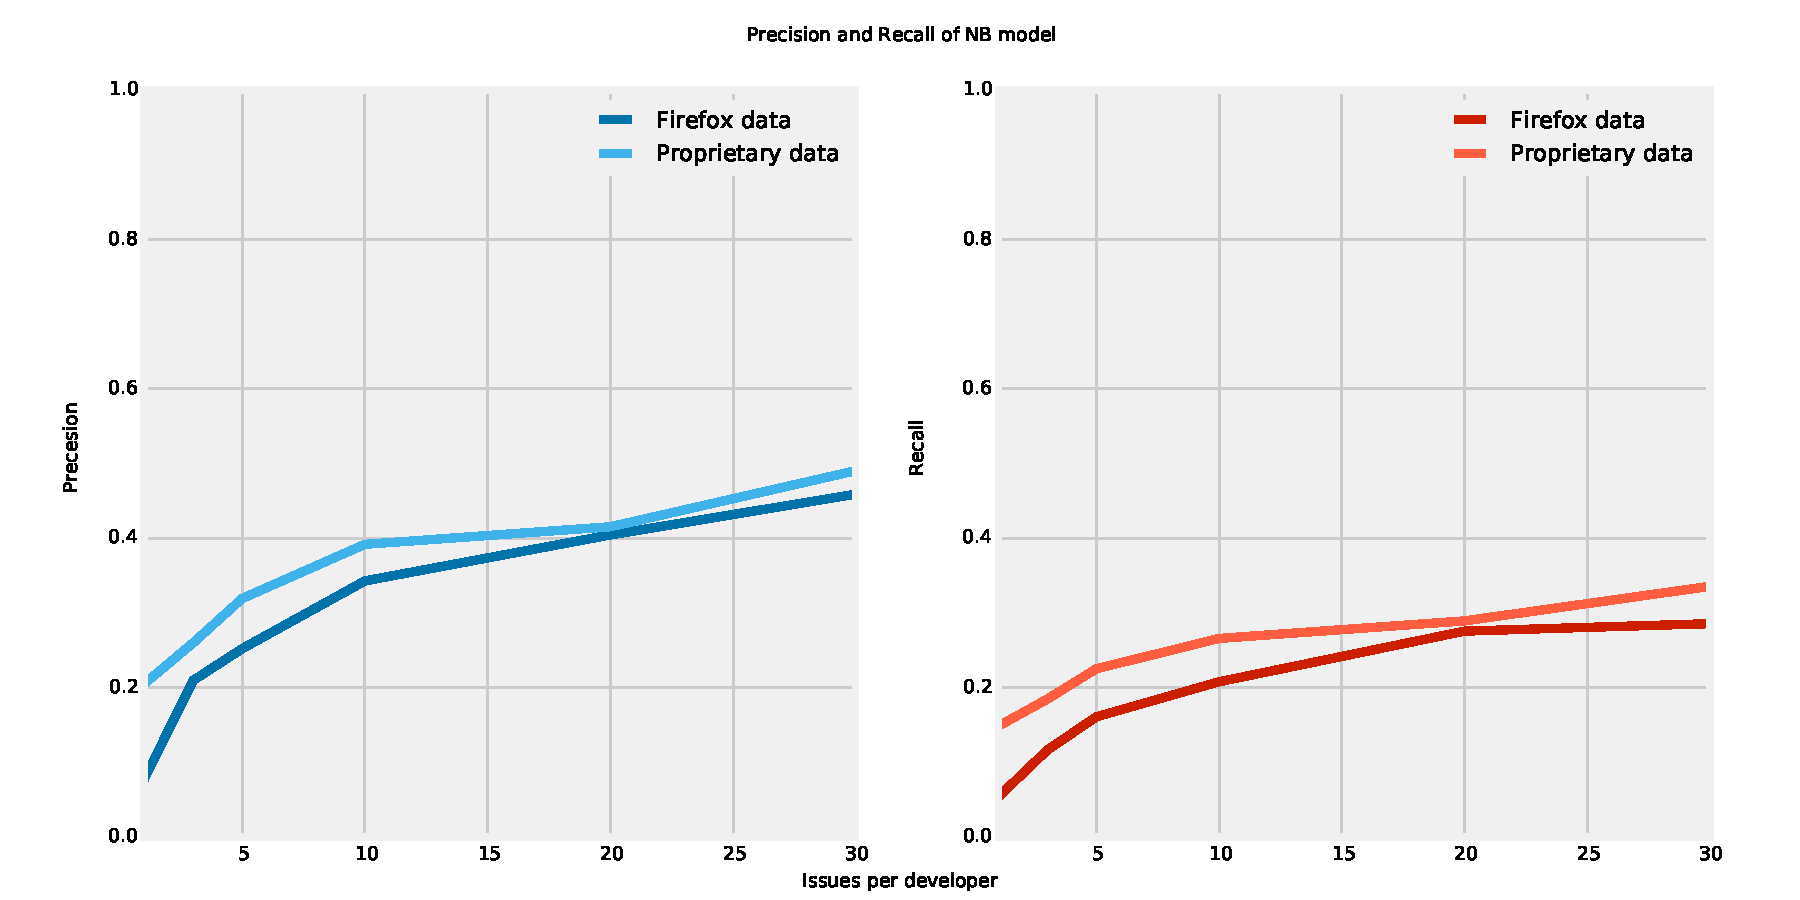
\includegraphics[width=\textwidth]{./images/prop_vs_os/nb_precision_and_recall.pdf}
    \caption{Comparison of precision and recall of Naive Bayes model.}
    \label{fig:results.datasets.nb_pr}
\end{figure}

Second plot (Figure \ref{fig:results.datasets.nb_pr}) shows the precision and recall values of the same model. Precision of the classifier for minimum issues per developer equal to 30 is 47\% and 49\% for the open source and proprietary data, respectively. Recall value is 29\% for the open source data and 33\% for the proprietary data in this settings. For minimum requirement of issues per developer from 1 to 10, we again see the interesting discrepancy observed in the accuracy plot. While the precision of the proprietary dataset begins with 20\%, the precision of the open-source begins with mere 7\%, almost three times lower. The difference between recall values is also staggering as it begins almost three times lower for the open-source dataset (14\% vs 5\%).

\subsection{Support Vector Machine Model}

The second model used for comparison of the proprietary dataset with the open-source dataset is Support Vector Machine model with TF--IDF weighing and stop-words removal as this model shows the most promising results.

Figure \ref{fig:results.datasets.svm_accuracy} visualizes accuracy comparison of the model. While the accuracy of the proprietary dataset (53\%) is a bit lower than the accuracy of the open-source dataset (54\%) when minimum issues per developer equals 30 and while the value of this measure is about the same for all different values of issues per developer greater than 10, it begins again significantly higher for the proprietary dataset (42\%) than the open-source dataset (29\%). This difference cannot even partially be explained the same way we explained it in the Naive Bayes case as the accuracy difference eventually clears.

\begin{figure}[htbp]
    \centering
        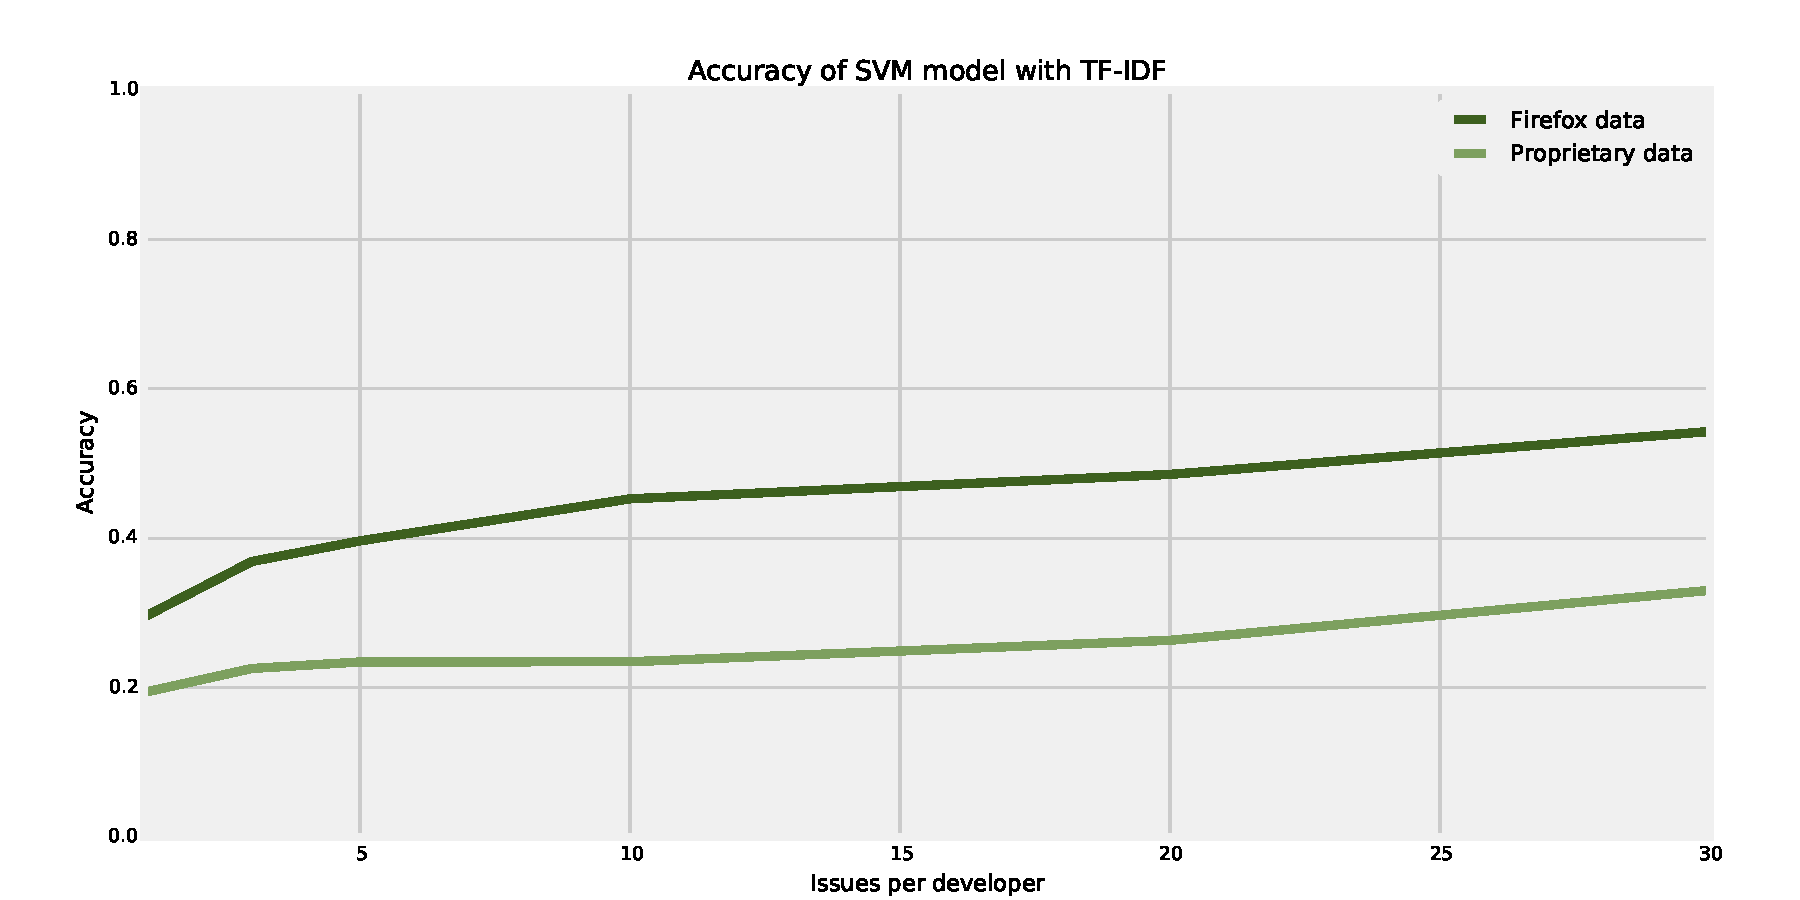
\includegraphics[width=\textwidth]{./images/prop_vs_os/svm_accuracy.pdf}
    \caption{Comparison of accuracy of SVM model.}
    \label{fig:results.datasets.svm_accuracy}
\end{figure}

Precision and recall of the SVM model is pictured on figure \ref{fig:results.datasets.svm_pr}. This plot, once again, confirms the hypothesis that the performance of the proprietary dataset begins much higher than the performance of the open-source dataset. The precision value of the proprietary dataset is eventually higher (59\%) than the precision value of the open-source dataset (54\%), but the difference at the beginning is just too overwhelming to be explained simply by the difference in performance overall (15\% vs mere 3\%). In the recall case, the right-most case (minimum number of issues per development requirement equal to 30) shows the performance of the proprietary dataset slightly lower (47\%) than that of the open-source dataset (50\%), even in this case, however, the performance for minimum number of issues per development equal to 1 is much higher for the proprietary dataset (14\% vs 3\%).

\begin{figure}[htbp]
    \centering
        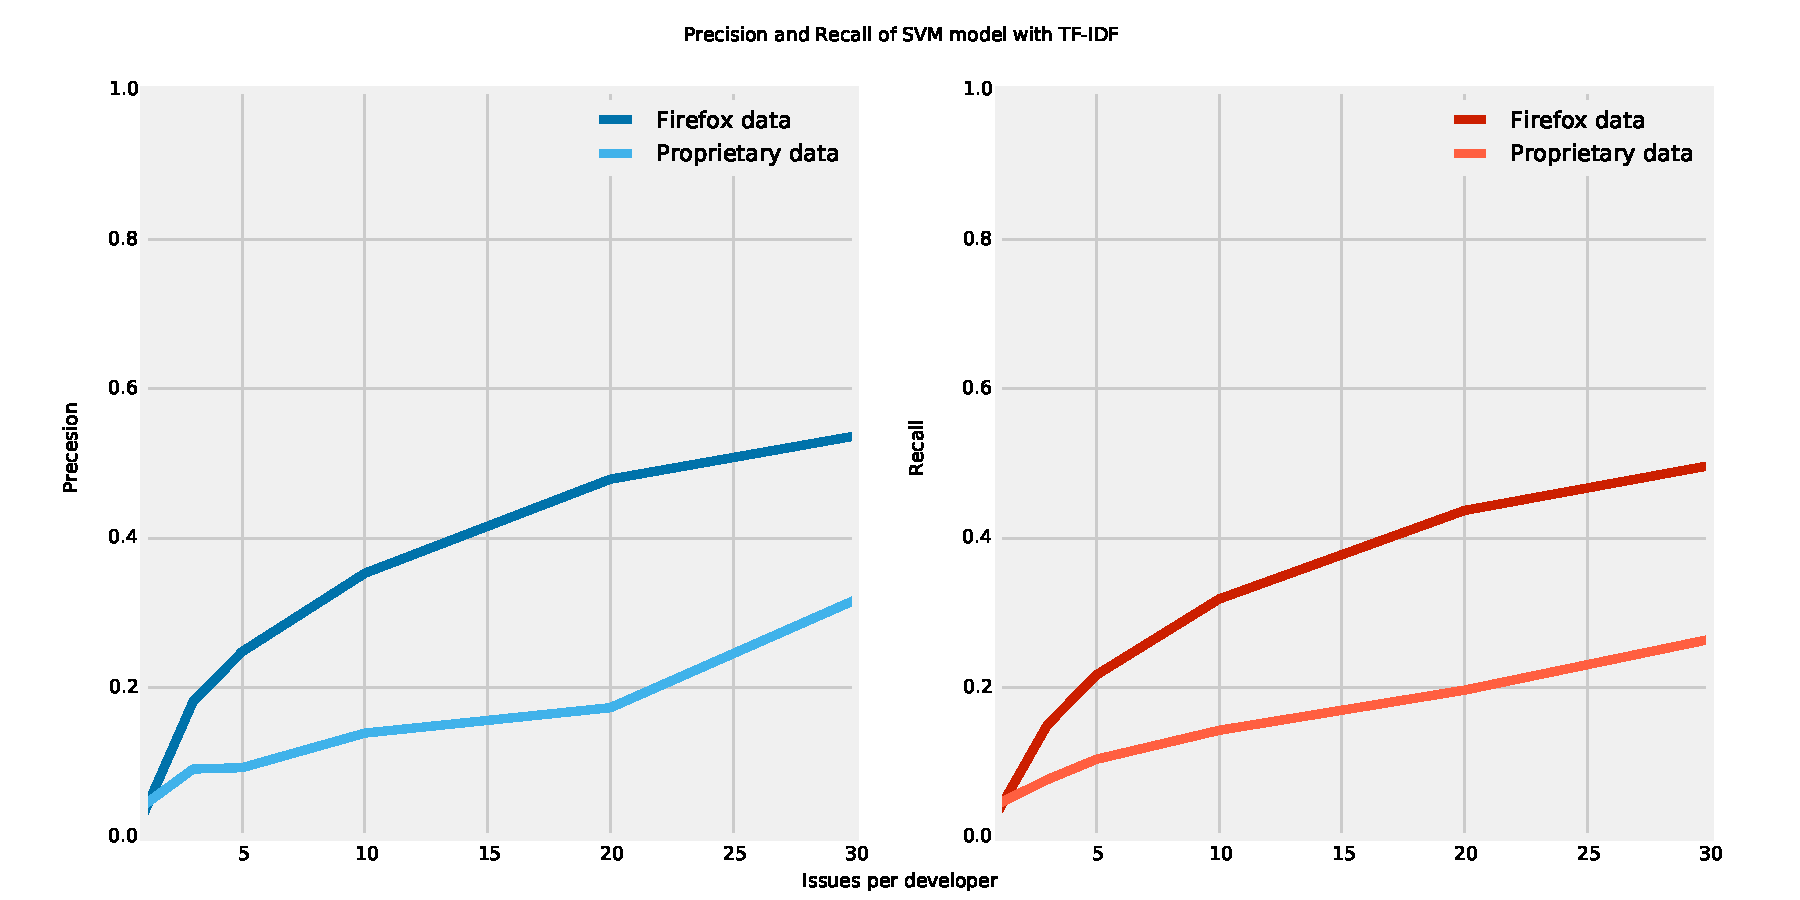
\includegraphics[width=\textwidth]{./images/prop_vs_os/svm_precision_and_recall.pdf}
    \caption{Comparison of precision of SVM model.}
    \label{fig:results.datasets.svm_pr}
\end{figure}

\subsection{Conclusion}

The results presented in this section suggest an interesting outcome. The performance of the proprietary dataset is generally quite similar to that of the open-source dataset at least as far as the accuracy of the SVM model is concerned. The Naive Bayes model seems to favor the proprietary dataset, however. Another interesting conclusion is that the spread between precision and recall is much higher for the proprietary dataset. This possibly implies higher variance of the dataset. The most striking result, however, emerges when the minimum number of issues per developers equals 1.

In terms of GQM defined in chapter~\ref{chapter:methodology}, we are now talking about question~\hyperlink{question:5}{5}. All our results show significant difference in performance for minimum number of issues per developers equal to 1. The much higher performance for the proprietary dataset in this regard can be probably explained by a simple fact---open-source bug repositories are open to anyone. It is logical to assume that a lot of bug reports in an open-source bug repository are fixed by random users that have never fixed bugs in the project, or fixed only a few of them---and only several users are actively maintaining the project. Proprietary projects are rarely open to public and it is therefore very unlikely there are many one-time assignees.

\section{Performance for Higher Number of Recommendations}
\label{section:compare-number-of-recommendations}

We look at the performance of the models for higher number of recommendations than one in this section. The plots will show the performance of the SVM model with TF-IDF weighing trained on the proprietary and Firefox datasets for number of recommendations from 1 to 10. In terms of GQM defined in chapter~\ref{chapter:methodology}, this section answers question~\hyperlink{question:7}{7}.

\subsection{Support Vector Machine Model}

For this comparison, we use the SVM model with TF-IDF weighing and stop-words removed. Figure \ref{fig:results.topx.svm_accuracy} shows how the accuracy increases with the number of recommendations, which is expected as the more there are recommendation, the higher the chance of a hit is.

\begin{figure}[htbp]
    \centering
        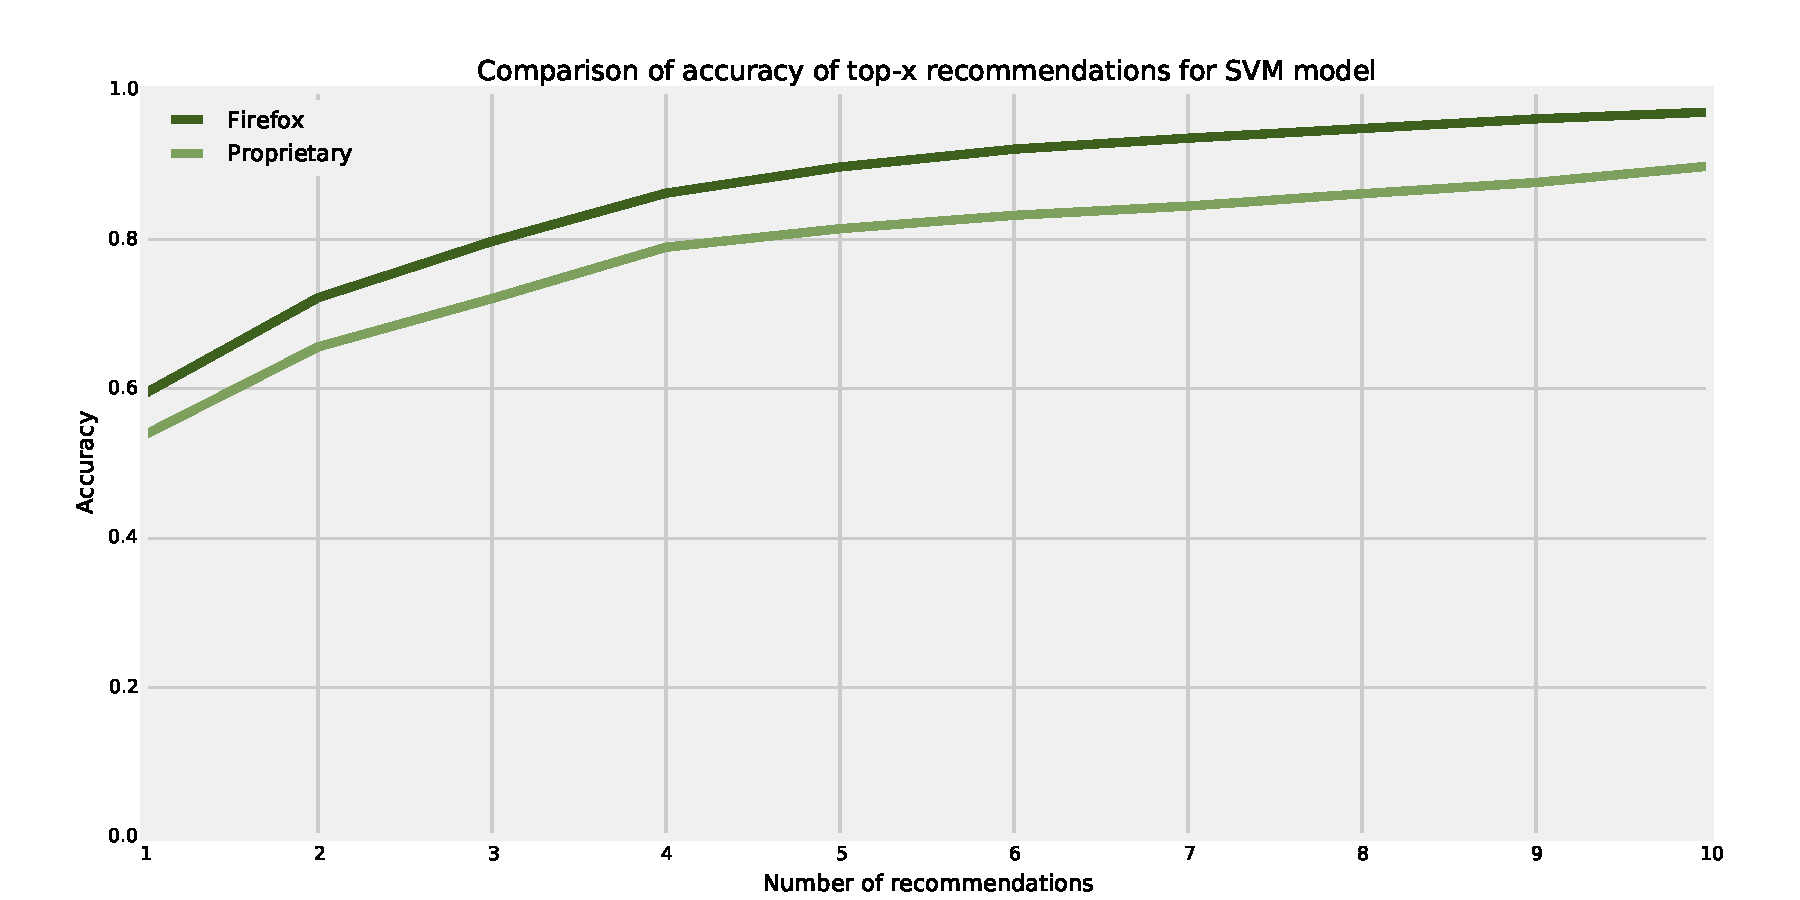
\includegraphics[width=\textwidth]{./images/top_x_comparison/svm_accuracy.pdf}
    \caption{Comparison of accuracy of top-x recommendations for SVM model.}
    \label{fig:results.topx.svm_accuracy}
\end{figure}

It is apparent from the plot that the highest performance boost happens when the number of recommendations changes from one to two both for the proprietary dataset (54\% vs 66\%) and the Firefox dataset (59\% vs 72\%). The accuracy of the Firefox dataset is equal to 90\% for 5 recommendations and 81\% for proprietary dataset. When the number of recommendations is 10, the performance is 97\% and 90\% for the Firefox and proprietary data respectively.

\subsection{Conclusion}

From the results in this section, we conclude that the highest number of recommendations to suggest to users that makes sense is 5. The performance does not increase very much with more recommendations and it would probably only lead to confusion if the number of recommendations was too high.

\section{Window Size}
\label{section:window-size}

The size of the time window is an important question that needs to be addressed when dealing with machine learning. A naive approach uses all samples from a dataset to train the classifier, but a more advanced approach considers what effect does the size of the window have on the data and how it can improve the performance. In this section, we try to address this concern by evaluating the performance of the classifier for different sizes of the window (addressing~\hyperlink{question:6}{Q6}).

To determine weather a different size of the window helps the performance is a difficult endeavour, we attempt it by employing three different approaches, each approach can be described by two properties:

\begin{enumerate}
 \item Fixed number of bugs per period, variable size of the train set
 \item Variable number of bugs per period, fixed size of the train set
 \item Variable number of bugs per period, variable size of the train set
\end{enumerate}

The Firefox dataset is used for testing of all approaches. The model that is applied is Support Vector Machine with TF--IDF weighing---the reason for this choice is clear in the evaluation part of this chapter, the choice, however, is not really important for the analysis.

\subsection{First Approach}

In the first approach, we first remove all bugs from the whole dataset that were fixed by developers with less than 20 fixed bugs. Then we split the remaining dataset into 8 bins. First bin contains 1000 randomly selected bug reports from period 1. All subsequent bins (2-8) contain 500 randomly selected reports from periods 2-8. There are 8 periods, first period is about one year long, all the other periods are about half a year long each. All periods combined add up to the time span of the whole dataset and each $n+1$ period contains bugs older than $n$ period. We train the classifier on period 1, then 1-2, 1-3, 1-4, 1-5, 1-6, 1-7 and 1-8. We test each trained classifier on the same cross-validation set of 300 bug reports that are newer than bugs in period 1.

The disadvantage of this approach is that you select fixed number of bugs from each period. In real world, each period can contain different number of bug reports based e.g. on season. Another disadvantage is that you remove developers that do not meet the criteria of 20 bugs fixed based on the whole dataset. If some developers were very active in the past but are no longer very relevant, they will not be removed from a dataset that is constructed from periods in which the developer no longer fulfills the criteria.

\begin{figure}[htbp]
    \centering
        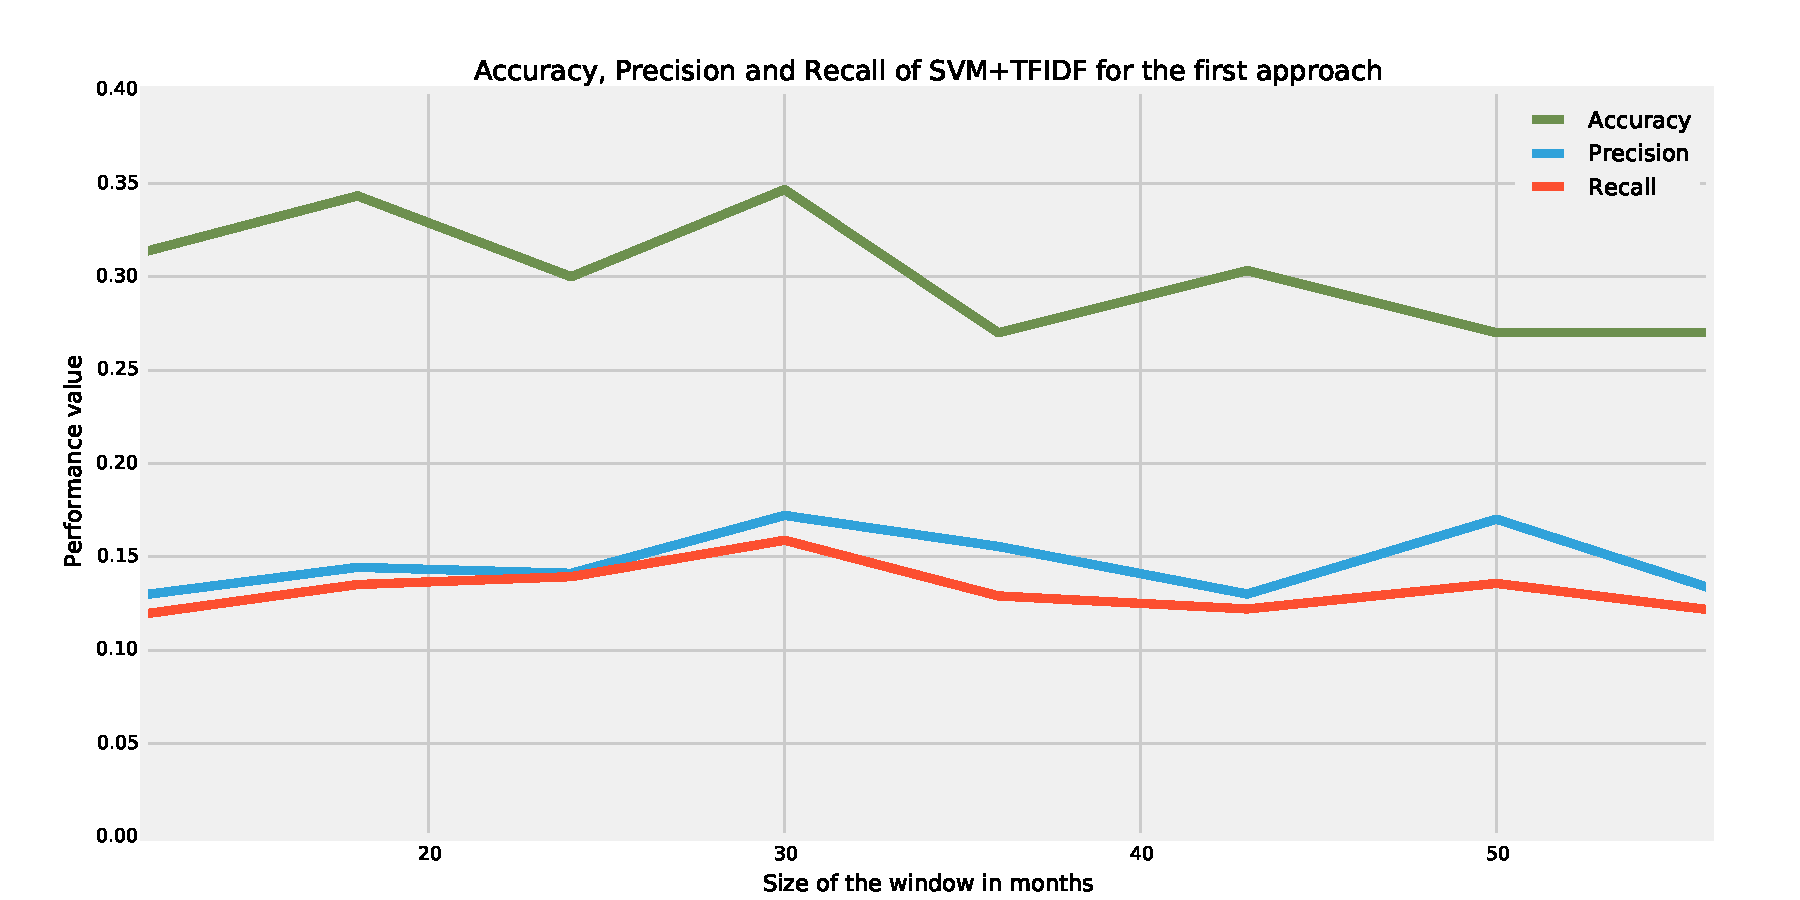
\includegraphics[width=\textwidth]{./images/window_size/firefox_1a.pdf}
    \caption{Performance of the classifier for different sizes of the window, 1st approach.}
    \label{fig:window.firefox.1a}
\end{figure}

The result is visualized on figure~\ref{fig:window.firefox.1a}. You can see that about the best result is achieved with the size of the window equal to 30 months. Unfortunately, the performance of the classifier for other sizes is very similar and the results are therefore inconclusive.

\subsection{Second Approach}

In the second approach, we employ the same periods, except period 1 that is about 15 months long. Another difference is that each train set contains 3000 randomly selected bug reports from period 1, 1-2, 1-3 etc. and the size of the sample is in this case therefore fixed, what is different is the period from which they were selected. From each bin, all bug reports that were fixed by a developer with less than 30 fixed bugs within the same train set are removed. We also remove all bug reports from cross-validation set that are not in the train set. We do this to get more relevant results from macro-averaged metrics, because otherwise the result of such metrics would be very close to zero.

The disadvantage of the second approach is that it does not really tell us what size of the window can be used to get the best performance. What it shows is whether the size of the window from which an equal size of sample is selected matters.

\begin{figure}[htbp]
    \centering
        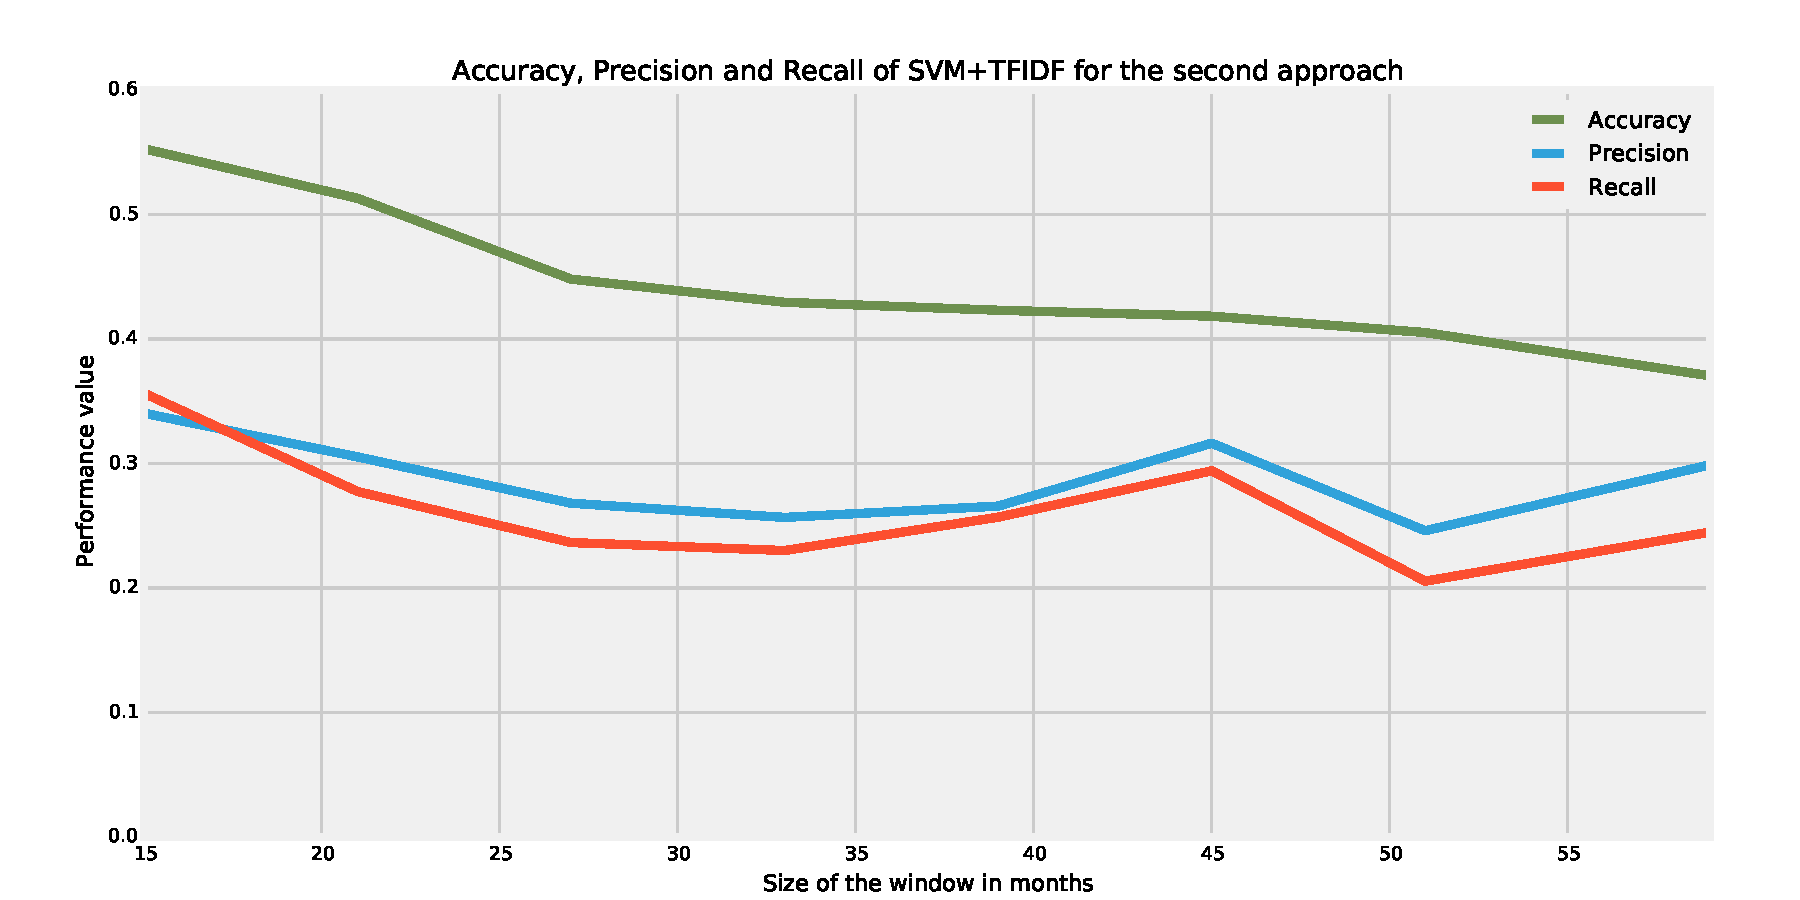
\includegraphics[width=\textwidth]{./images/window_size/firefox_2a.pdf}
    \caption{Performance of the classifier for different sizes of the window, 2nd approach.}
    \label{fig:window.firefox.2a}
\end{figure}

Figure~\ref{fig:window.firefox.2a} shows the plot of this approach. The performance decreases as the size of the window increases, which is expected. Precision and recall however increases when the size of the window is around 45 months.

\subsection{Third Approach}

Finally, in the third approach, we again use the same periods as in the second approach. The difference is that we select all bug reports as train set. The advantage is that this approach is closest to reality (no random selection). The disadvantage is, however, that the results are skewed by a variable number of samples in each period. The last major disadvantage is that the number of classes (developers) increases significantly each time samples from the next period are added. Figure~\ref{fig:window.firefox.3a} shows the plot of this approach.

\begin{figure}[htbp]
    \centering
        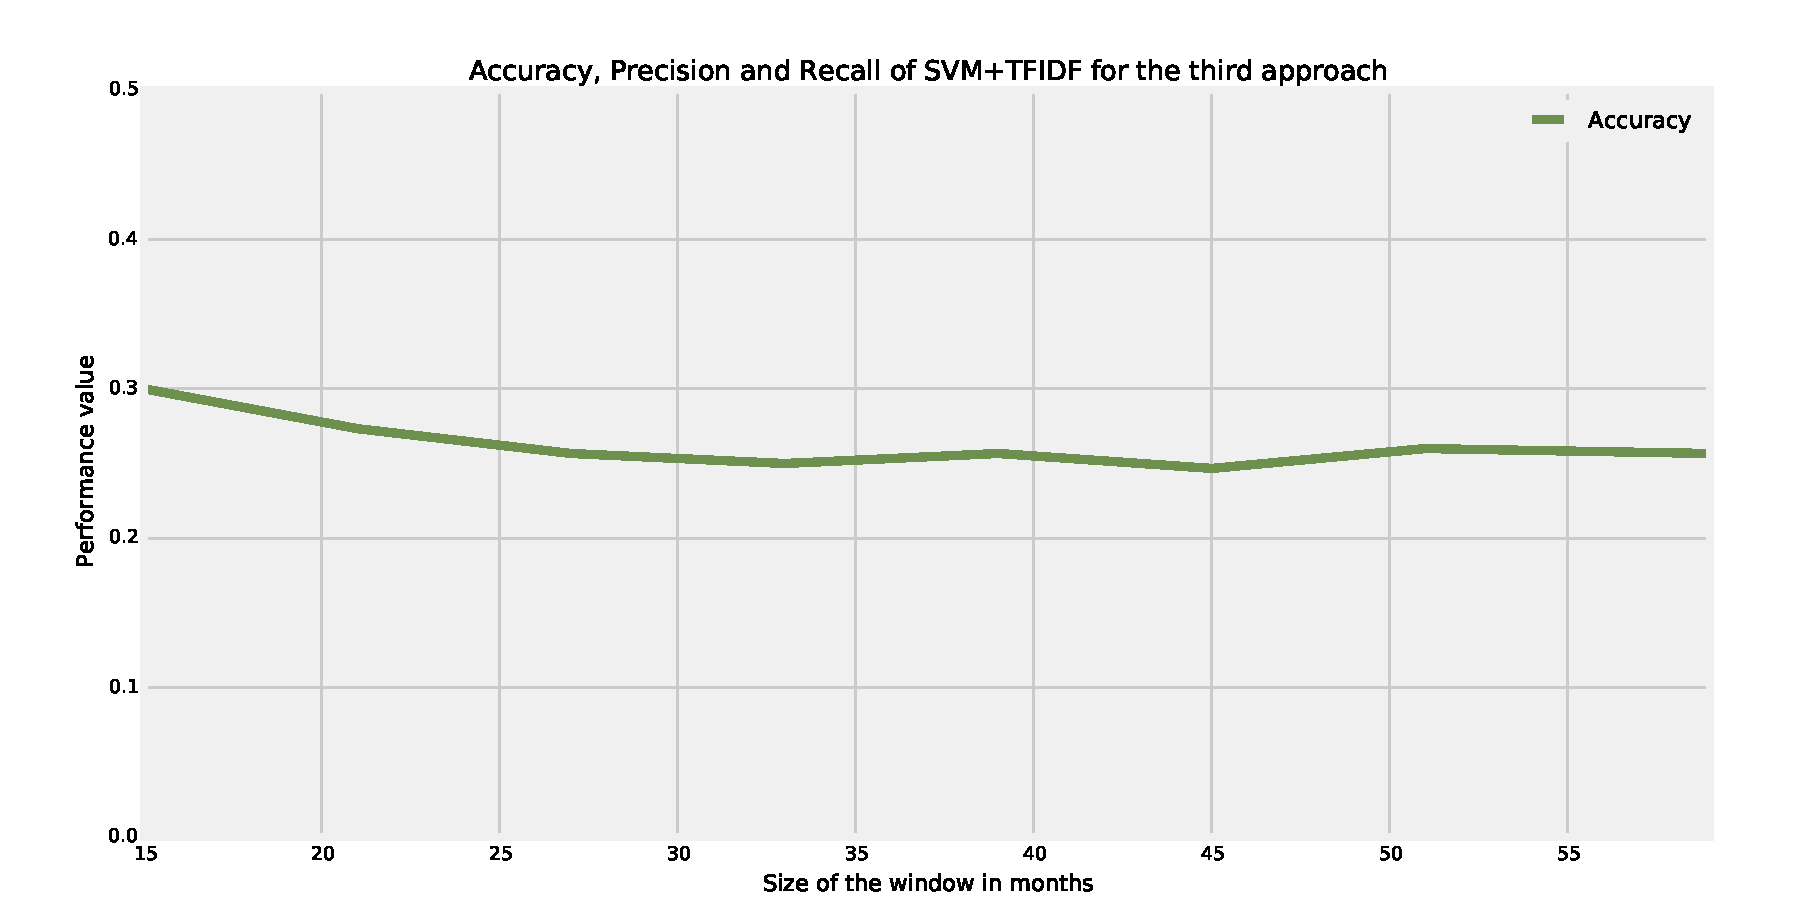
\includegraphics[width=\textwidth]{./images/window_size/firefox_3a.pdf}
    \caption{Performance of the classifier for different sizes of the window, 3rd approach.}
    \label{fig:window.firefox.3a}
\end{figure}

\subsection{Conclusion}

Even after the application of all three approaches, it is hard to draw a concrete conclusion about the window size effect on the performance. The results do seem to imply that there are no significant differences in terms of performance between different time-windowing strategies (\hyperlink{question:6}{Q6}), but to increase the confidence of these results, it would be necessary to do a more thorough analysis with possibly more approaches or different processing strategy.

\section{Topic Analysis}

In this section, we analyze the distribution of topics with respect to time for proprietary and Firefox datasets in order to further determine the differences or similarities of open-source and proprietary datasets. We model 10 topics using Latent Dirichlet Allocation (LDA) in our approach.

The plots show the prevalence of topics each month where a different shade of gray represents a different topic. In terms of our GQM methodology, this section contributes to the answer of questions~\hyperlink{question:4}{4} and~\hyperlink{question:5}{5} (described in chapter~\ref{chapter:methodology}).

\subsection{Firefox Data}

We begin our topic analysis with the Firefox dataset. All our Firefox bug reports were created within 62 months (about 5 years). You can see the distribution on figure~\ref{fig:distribution.firefox.topic}.

\begin{figure}[htbp]
    \centering
        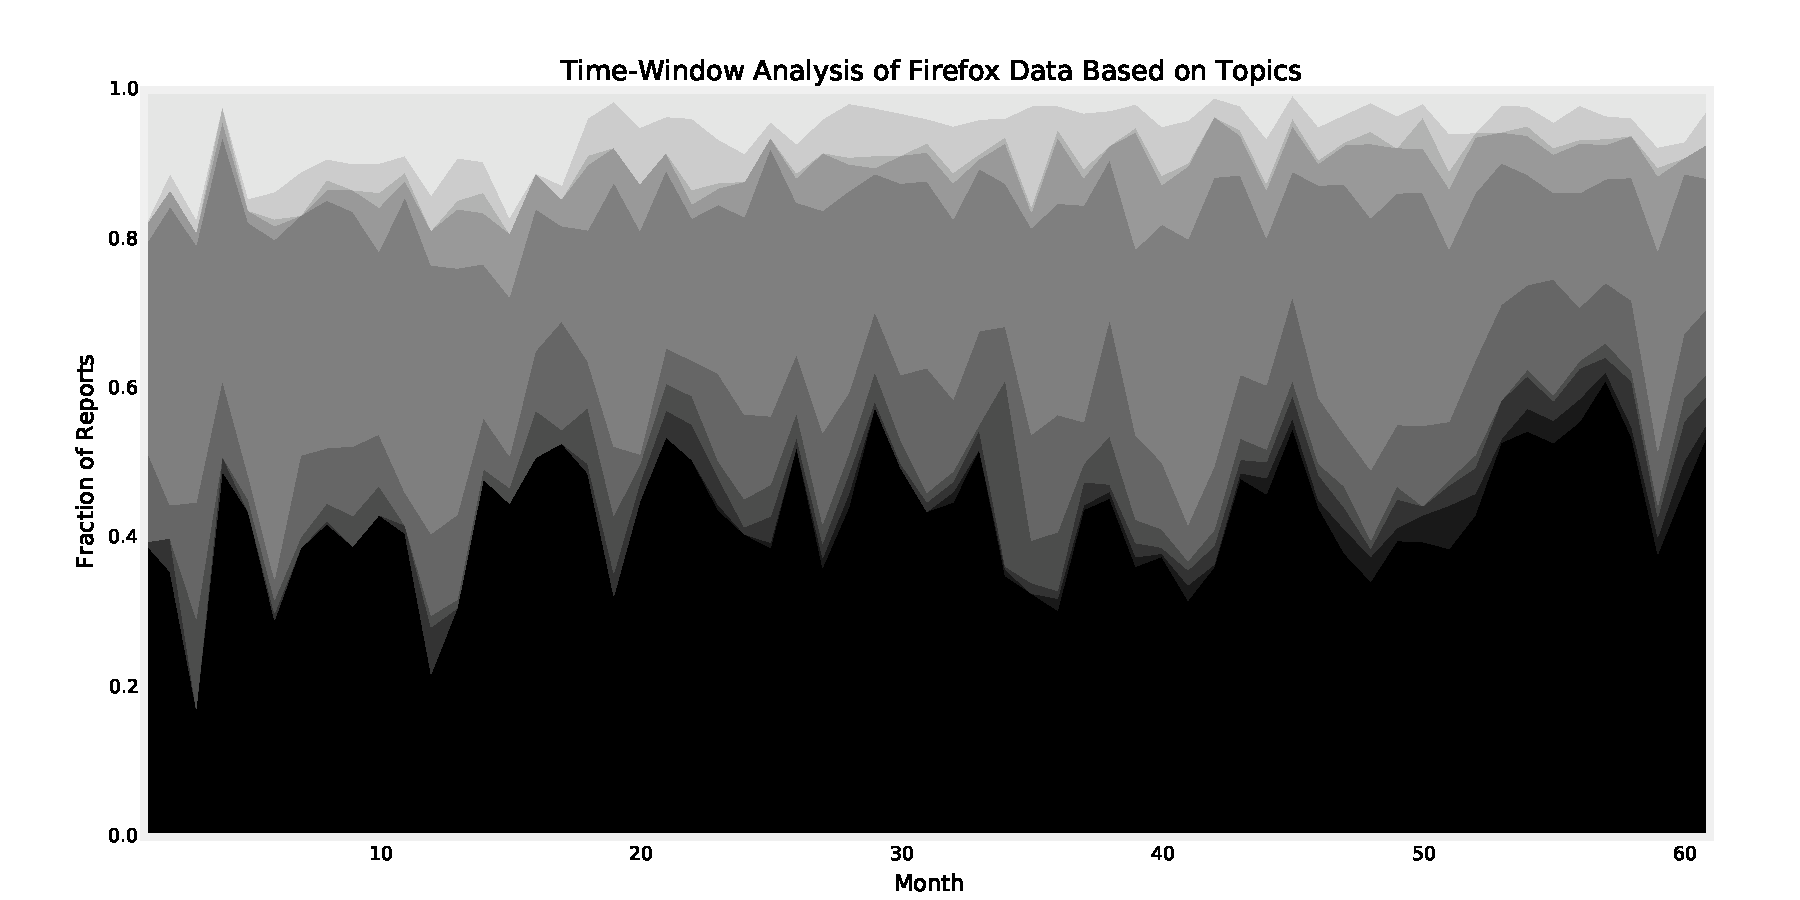
\includegraphics[width=\textwidth]{./images/topic_component_distribution/firefox_topic_10.pdf}
    \caption{Topic analysis of Firefox data.}
    \label{fig:distribution.firefox.topic}
\end{figure}

The plot shows that the distribution of topics is quite significantly different each month with two dominant topics. The distribution of the topics seems to oscillate periodically which could be an indication of a release cycle of major Firefox versions, which would not be surprising as many projects have a predetermined periodic release cycle.

\subsection{Proprietary Data}

The proprietary bug reports were created within 36 months. You can see the distribution on figure~\ref{fig:distribution.prop.topic}. The plot again shows that the distribution of topics in the proprietary datasets is quite different each month, although their dominance changes quite a lot as well. The first few months are dominated by a single topic, but its significance later drops as other topics take over. Contrary to the Firefox distribution, there does not seem to be an indication of a release cycle, instead, each topic seems to be important only for a limited period of time.

\begin{figure}[htbp]
    \centering
        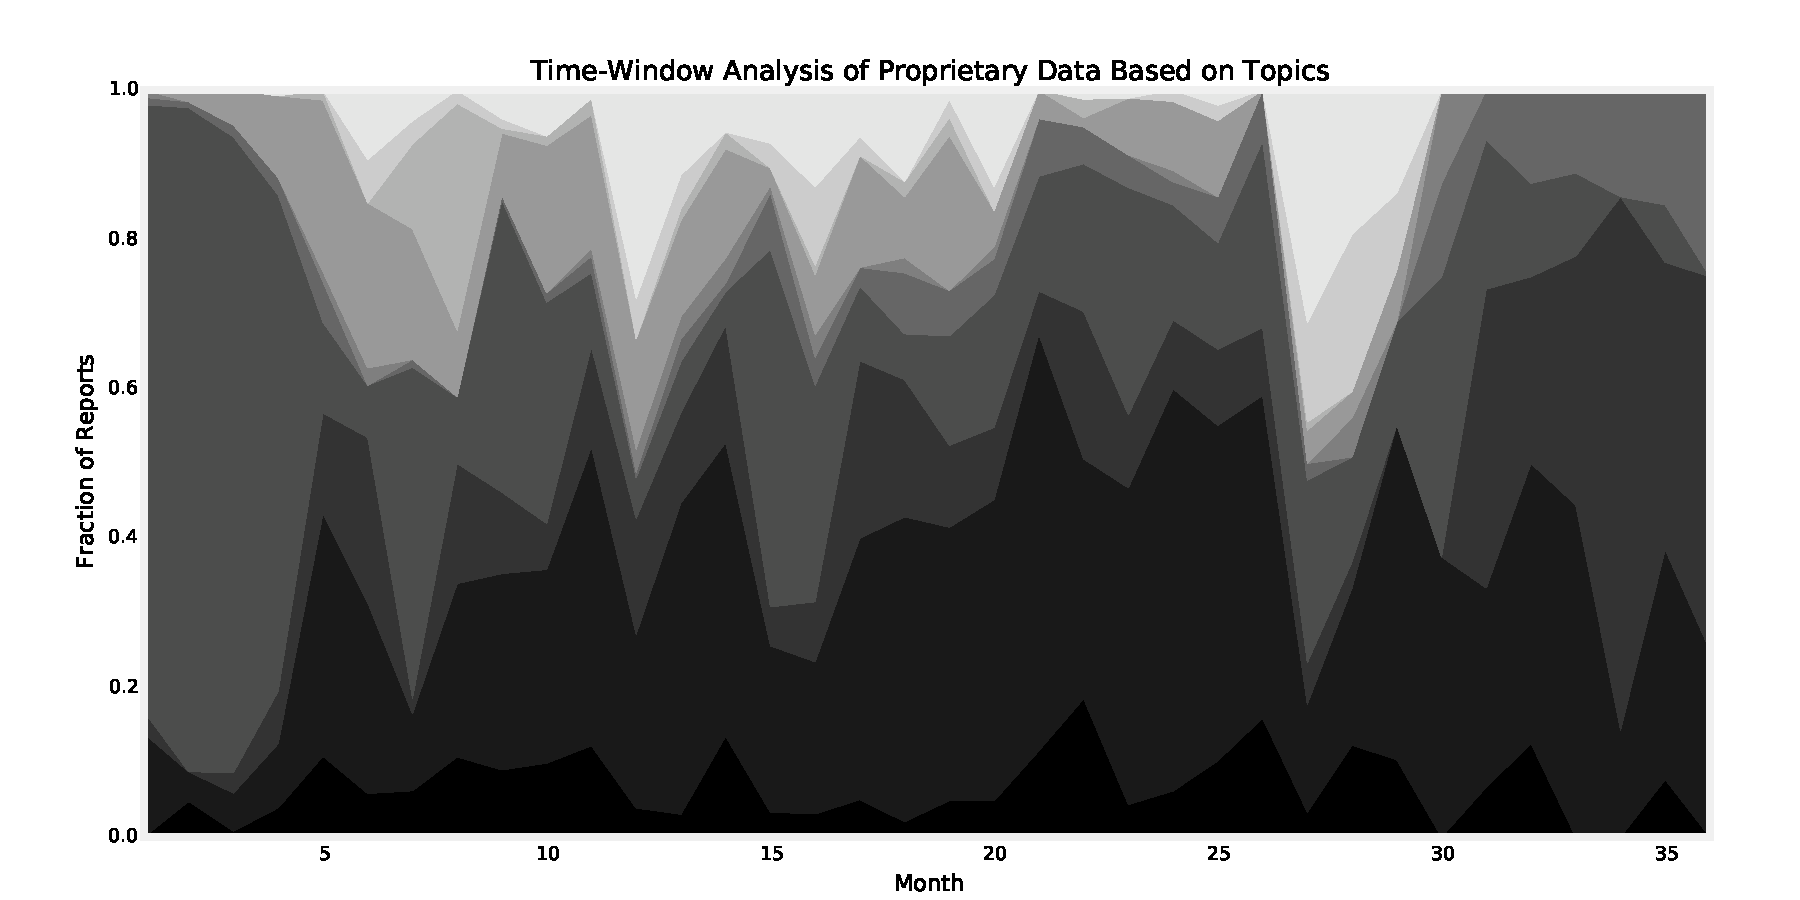
\includegraphics[width=\textwidth]{./images/topic_component_distribution/proprietary_topic_10.pdf}
    \caption{Topic analysis of the proprietary data.}
    \label{fig:distribution.prop.topic}
\end{figure}

\subsection{Conclusion}

The topic analysis presented in this section does suggest some difference in topic distribution (with respect to time). It is not surprising as different projects are developed different ways, the application of different software development methodologies (scrum, waterfall, TDD etc) is one of the factors that are likely to affect the results. In terms of~\hyperlink{question:4}{Q4}, these results decrease our confidence that our models work for all datasets equally without the need to tune their parameters. As far as~\hyperlink{question:5}{Q5} is concerned, the difference between the Firefox and proprietary datasets can be explained by different development processes.

In this chapter, we presented the results for our analysis and our evaluation. In the next chapter, we discuss the results in greater detail. We also compare them with the related work and disucuss some possible threats to their validity. 
